\clearpage
\begin{savequote}[8cm]
\textlatin{Neque porro quisquam est qui dolorem ipsum quia dolor sit amet, consectetur, adipisci velit...}

There is no one who loves pain itself, who seeks after it and wants to have it, simply because it is pain...
  \qauthor{--- Cicero's \textit{de Finibus Bonorum et Malorum}}
\end{savequote}

\chapter{\label{ch:6-backgrounds}Backgrounds} 

\minitoc

\section{Backgrounds}
\label{sec:backgrounds}

\subsection{Partially reconstructed $B \to D^*K^*$ decays}
\label{sec:backgrounds:partreco}

One of the major backgrounds in this analysis is from partially reconstructed \decay{\B}{\Dstar\Kstar} decays, discussed in detail in Section \ref{sec:massfit:partreco} and included in the mass fit.

\subsection{Charmless backgrounds $B \to K^*hh$}
\label{sec:backgrounds:charmless}

\B decays that do not proceed via a \D meson contribute to the charmless background. This is a peaking background under the signal region which is expected to be uniform in \D mass. The flight distance significance of the \Dz in the z direction is defined as,

\begin{equation}
\Dz\ FD\ significance = \frac{z_D - z_B}{\sqrt{\sigma_D^2 + \sigma_B^2}}
\label{FDdefinition}
\end{equation}

where, $\sigma_D$ and $\sigma_B$ are the errors in the z position of the \D and \B decay vertex respectively. This background is removed by requiring \Dz FD significance to exceed 2$\sigma$. The charmless background is estimated and removed by taking the D mass sidebands ($>$ 50 MeV from nominal \D mass) in data and performing a fit to the invariant \B mass distribution. In order to correctly estimate the background contribution in the \D sidebands all DTF variables are replaced in the selection as the use of these variables favours events towards the true \D mass. In the BDTs the DTF vertex $\chi^2$ fit is replaced with the non-DTF version. This fit to data is performed with a FD significance cut of both zero and 2$\sigma$, as shown in Figure \ref{charmlesspipi}. Corresponding plots for all the modes are given Appendix \ref{sec:app:charmless}.

\begin{figure}
\centering
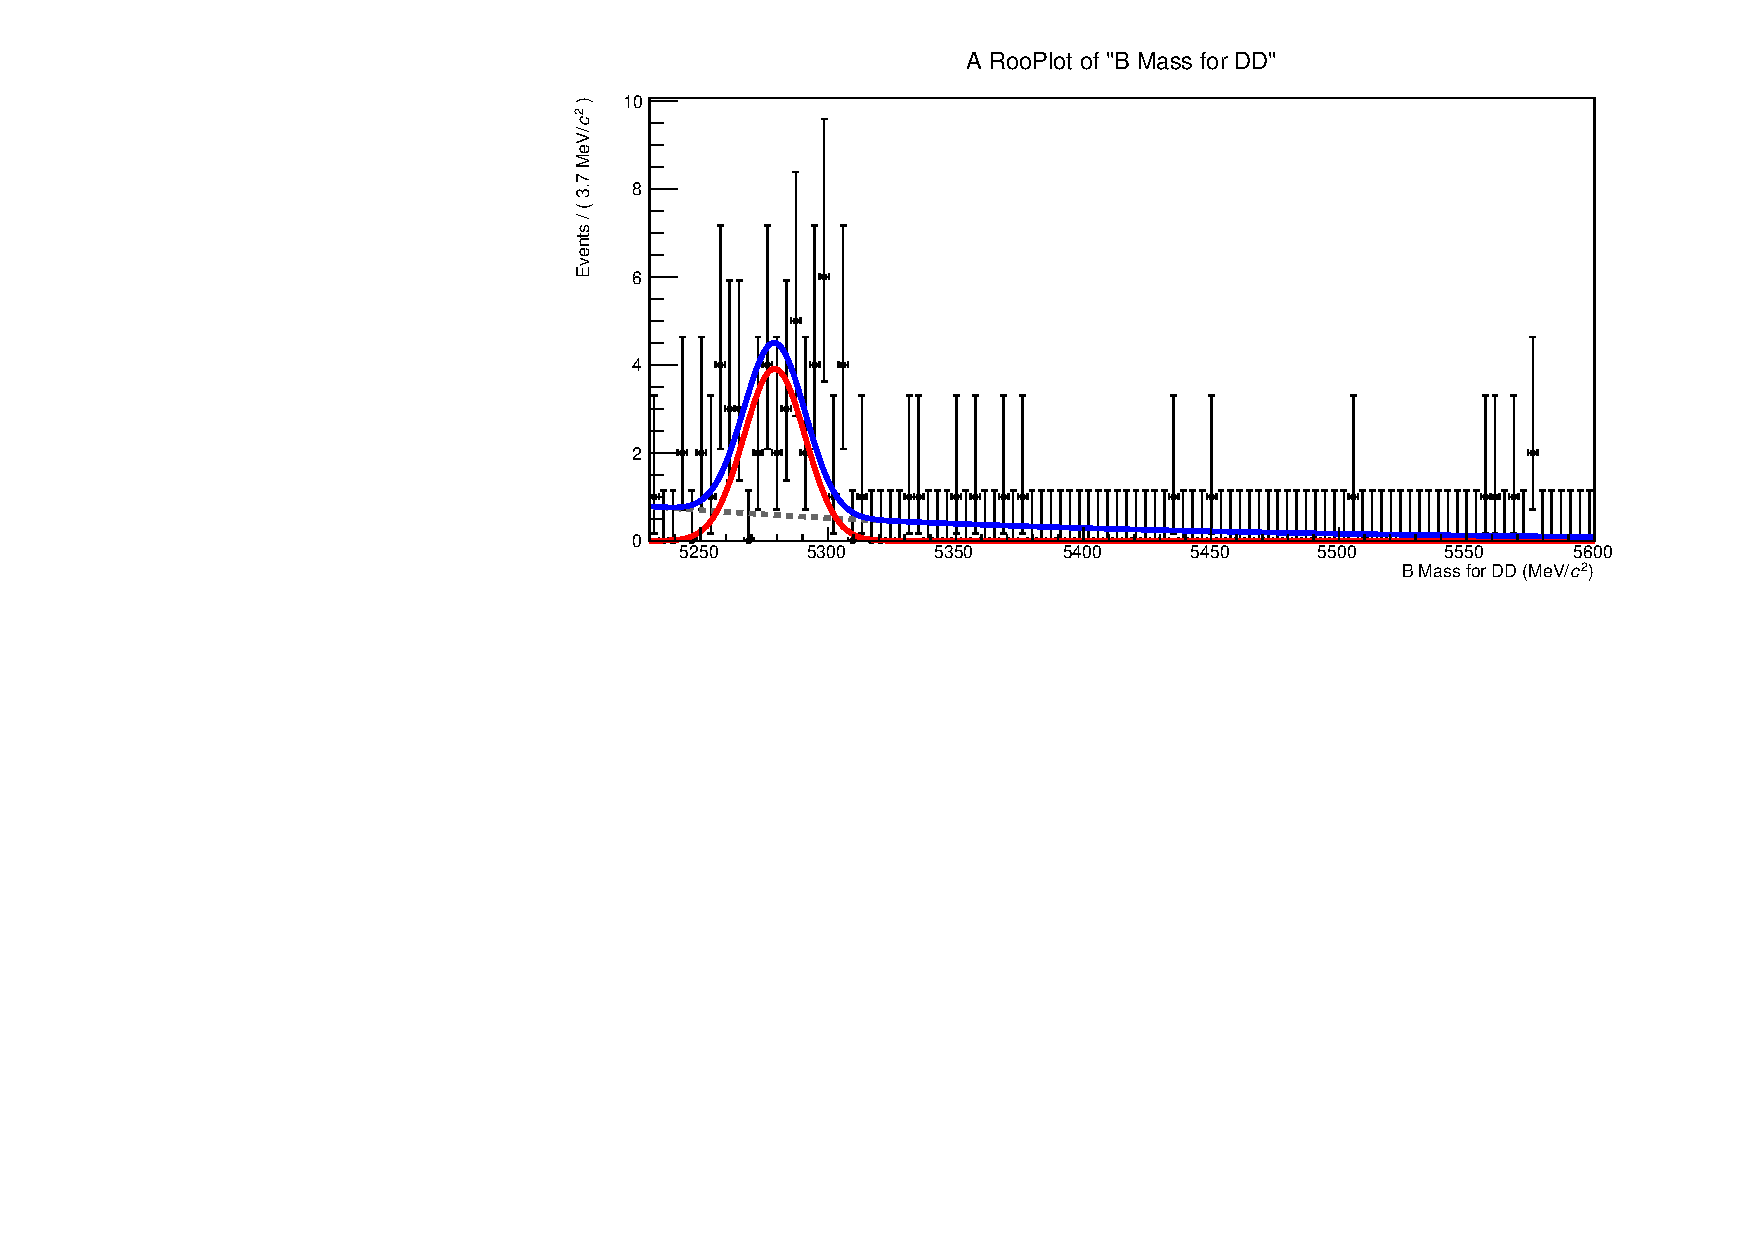
\includegraphics[width=0.7\linewidth]{figures/backgrounds/charmlessFit_PiPi_DD_FD0.pdf}
\put(-100,100) {(a)}
\hfill
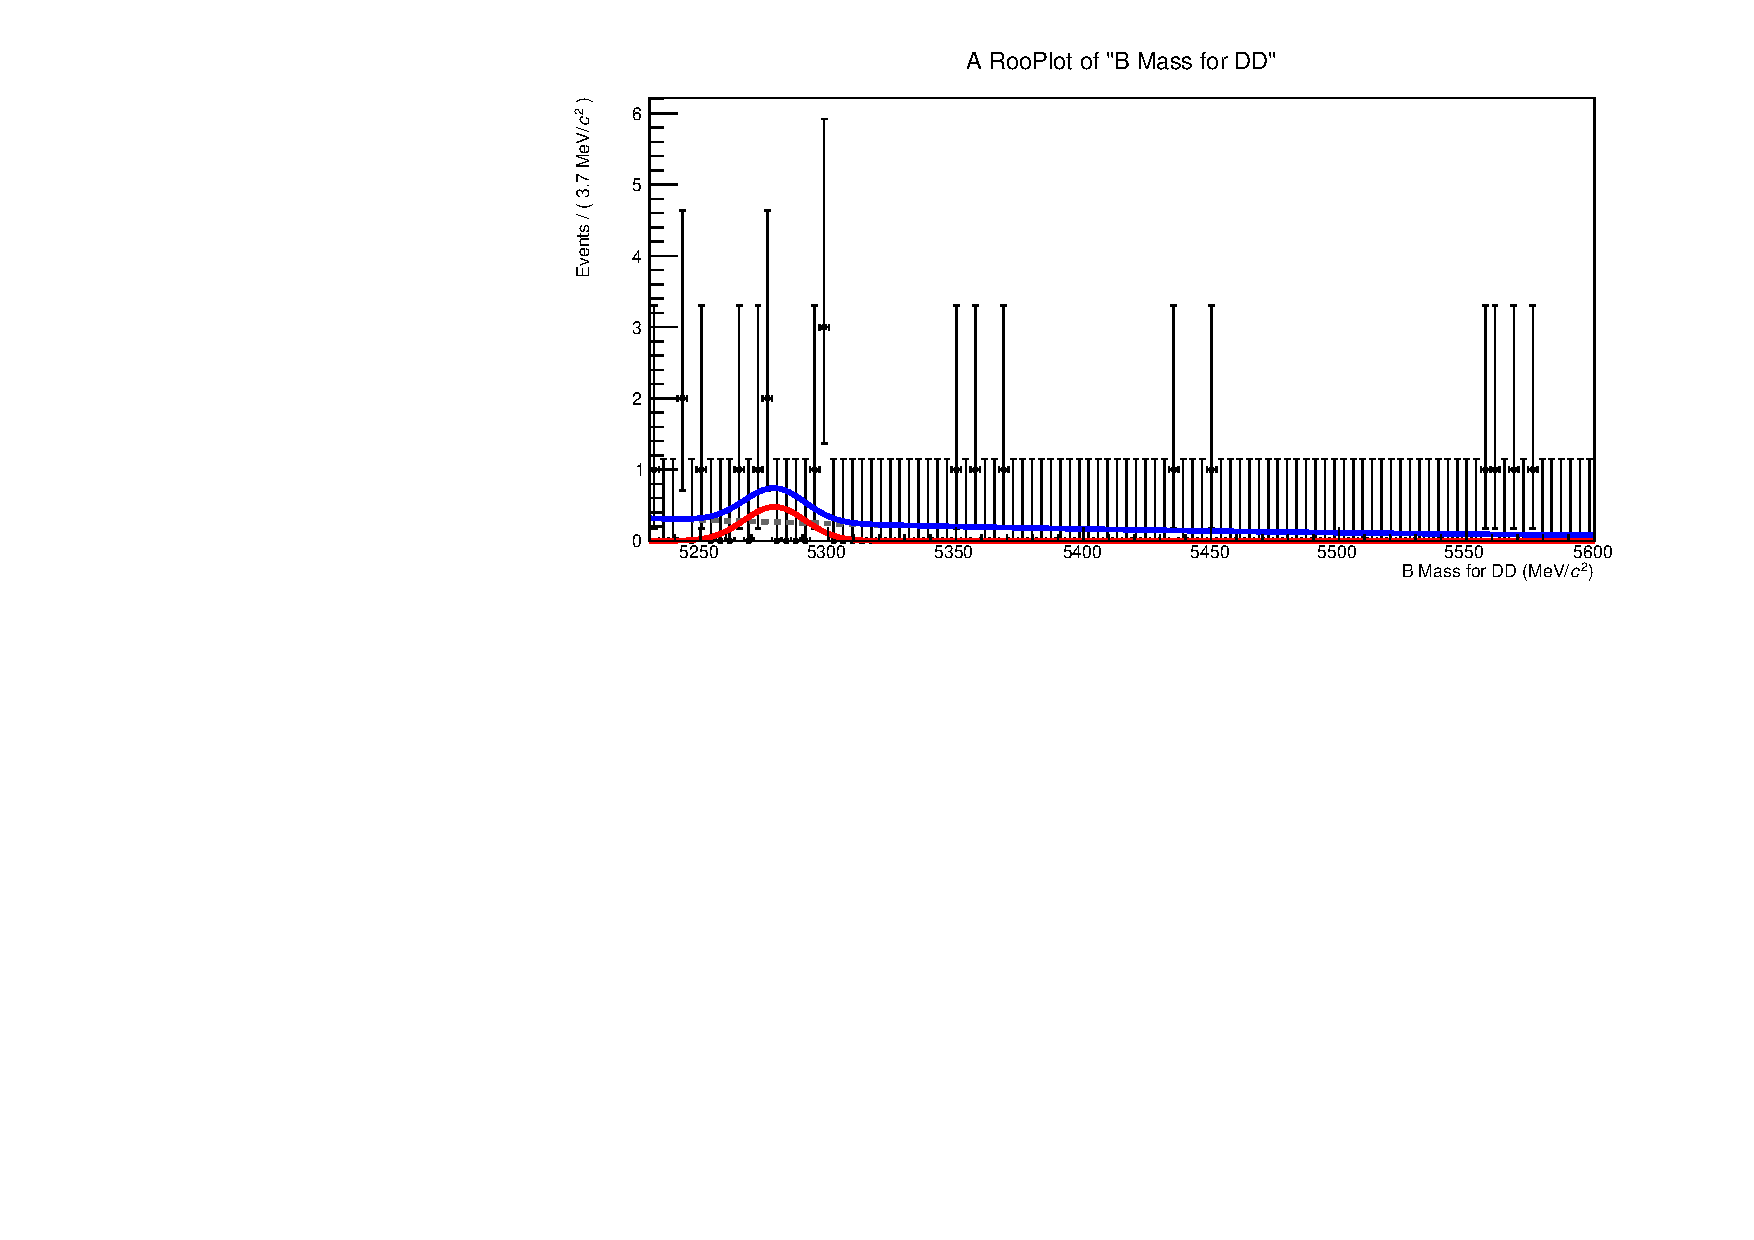
\includegraphics[width=0.7\linewidth]{figures/backgrounds/charmlessFit_PiPi_DD_FD2.pdf}
\put(-100,100) {(b)}
\caption{Fits to the Run 1 refitted B mass taking \decay{\Dz}{\pi\pi} candidates from the D mass sidebands after a FD significance cut (a) greater than 0 and (b) greater than 2$\sigma$. A Gaussian is used to model the signal and an exponential for the combinatoric background.}
\label{charmlesspipi}
\end{figure}

The yield of the \B mass peak is measured in the \D mass sidebands and then scaled to the \D mass window. This gives an estimate of the charmless yields expected after selection in the mass fit. These fits are performed using Run 1 data both with a FD significance cut of zero and a 2$\sigma$ FD cut applied, the resulting yields estimates are shown in Tables \ref{charmlessyieldsnofd} and \ref{charmlessyields} respectively. The same fits were peformed on Run 2 data and the results for the estimated charmless contribution in Run 2 for a zero and 2$\sigma$ FD cut, these are given in Tables \ref{charmlessyieldsnofdRun2} and \ref{charmlessyieldsRun2}.

\begin{table}[h] 
\centering 
\begin{tabular}{lll} 
\hline 
Mode & LL & DD \\ 
\hline 
$K\pi$ & $2.8 \pm 1.6$ & $2.6 \pm 1.9$ \\ 
$KK$ & $1.2 \pm 2.0$ & $0.6 \pm 2.2$ \\ 
$\pi\pi$ & $4.1 \pm 2.5$ & $16 \pm 4$ \\ 
$\pi K$ & $2.0 \pm 1.3$ & $0.0 \pm 0.6$ \\ 
$K\pi\pi\pi$ & $1.4 \pm 1.2$ & $1.5 \pm 2.0$ \\ 
$\pi\pi\pi\pi$ & $2.2 \pm 2.4$ & $6.8 \pm 3.5$ \\ 
$\pi K \pi\pi$ & $1.1 \pm 0.9$ & $1.3 \pm 1.2$ \\ 
\hline 
\end{tabular}
\caption{Estimated charmless contribution in Run 1 data for each of the D decay modes with a FD significance cut of zero applied} 
\label{charmlessyieldsnofd} 
\end{table}

\begin{table}[h]
\centering
\begin{tabular}{lll} 
\hline 
Mode & LL & DD \\ 
\hline 
$K\pi$ & $1.7 \pm 1.0$ & $0.2 \pm 1.6$ \\ 
$KK$ & $0.0 \pm 0.4$ & $0.0 \pm 0.4$ \\ 
$\pi\pi$ & $1.2 \pm 1.5$ & $2.0 \pm 1.6$ \\ 
$\pi K$ & $1.0 \pm 0.9$ & $0.0 \pm 0.3$ \\ 
$K\pi\pi\pi$ & $1.3 \pm 1.1$ & $0.1 \pm 3.7$ \\ 
$\pi\pi\pi\pi$ & $0.0 \pm 7.4$ & $0.0 \pm 1.2$ \\ 
$\pi K \pi\pi$ & $0.9 \pm 0.7$ & $0.0 \pm 0.7$ \\ 
\hline 
\end{tabular}
\caption{Estimated charmless contribution in Run 1 data for each of the D decay modes with a FD significance cut of 2$\sigma$ applied}
\label{charmlessyields}
\end{table}

\begin{table}[h] 
\centering 
\begin{tabular}{lll} 
\hline 
Mode & LL & DD \\ 
\hline 
$K\pi$ & $0.0 \pm 0.4$ & $0.0 \pm 1.6$ \\ 
$KK$ & $5.2 \pm 2.6$ & $7.1 \pm 4.0$ \\ 
$\pi\pi$ & $11 \pm 4$ & $30 \pm 5$ \\ 
$\pi K$ & $0.2 \pm 2.8$ & $1.1 \pm 1.7$ \\ 
$K\pi\pi\pi$ & $0.3 \pm 2.7$ & $1.6 \pm 3.3$ \\ 
$\pi\pi\pi\pi$ & $7.0 \pm 3.4$ & $8.7 \pm 5.3$ \\ 
$\pi K \pi\pi$ & $0.0 \pm 2.3$ & $0 \pm 17$ \\ 
\hline 
\end{tabular} 
\caption{Estimated charmless contribution in Run 2 data for each of the D decay modes with a FD significance cut of zero applied} 
\label{charmlessyieldsnofdRun2} 
\end{table}

\begin{table}[h] 
\centering 
\begin{tabular}{lll} 
\hline 
Mode & LL & DD \\ 
\hline 
$K\pi$ & $0.0 \pm 0.3$ & $0.6 \pm 1.3$ \\ 
$KK$ & $0.0 \pm 0.3$ & $0.0 \pm 0.7$ \\ 
$\pi\pi$ & $0.0 \pm 1.2$ & $2.3 \pm 2.2$ \\ 
$\pi K$ & $0.4 \pm 1.0$ & $0.0 \pm 0.5$ \\ 
$K\pi\pi\pi$ & $1.0 \pm 1.4$ & $0.0 \pm 7.6$ \\ 
$\pi\pi\pi\pi$ & $1.4 \pm 2.3$ & $0.0 \pm 1.0$ \\ 
$\pi K \pi\pi$ & $0.0 \pm 10.6$ & $1.4 \pm 1.5$ \\ 
\hline 
\end{tabular} 
\caption{Estimated charmless contribution in Run 2 data for each of the D decay modes with a FD significance cut of 2$\sigma$ applied} 
\label{charmlessyieldsRun2}
\end{table}

The \Dz FD significance is required to exceed 2$\sigma$, therefore from Tables \ref{charmlessyields} and \ref{charmlessyieldsRun2} it can be seen that all charmless contributions are consistent with zero. The expected yields in the $K\pi$ favoured and $KK$ modes are significantly less than 1\% of the expected signal yield. However, the charmless contribution in the $\pi\pi$ mode could be significant. A systematic is assigned to the possible charmless contribution in the $\pi\pi$ mode, details are given in Section \ref{sec:systematics}. 

\subsection{\decay{\B}{\D\pi\pi\pi}}
\label{sec:backgrounds:b2dpipipi}

\decay{\B}{\D\pi\pi\pi} decays, with a branching fraction of $5.7 \times 10^{-3}$~\cite{PDG2014} (about 50 times the signal branching fraction), are expected to occur as a peaking background underneath the signal. In order to remove this background, events are selected with the requirement that the \KS has flown. For DD candidates this requirement is already satisfied, however for LL candidates the flight distance significance of the \KS in the z direction, with the equivalent definition as for \Dz given in Equation \ref{FDdefinition}, is required to exceed 5$\sigma$. 

The \decay{\B}{\D\pi\pi\pi} background is removed by taking the \KS mass sidebands ($>$ 20 MeV from nominal \KS mass) in data and performing a fit to the invariant \B mass distribution. All DTF variables are replaced in the selection as descibed in Section \ref{sec:backgrounds:charmless}. This fit to data is performed for the favoured \decay{\Dz}{\Km\pip} mode with a FD significance cut of both zero and 5$\sigma$, as shown in Figure \ref{strangelessfits}. It can be seen that the 5$\sigma$ FD significance selection removes all of the \decay{\B}{\D\pi\pi\pi} background.

\begin{figure}
\centering
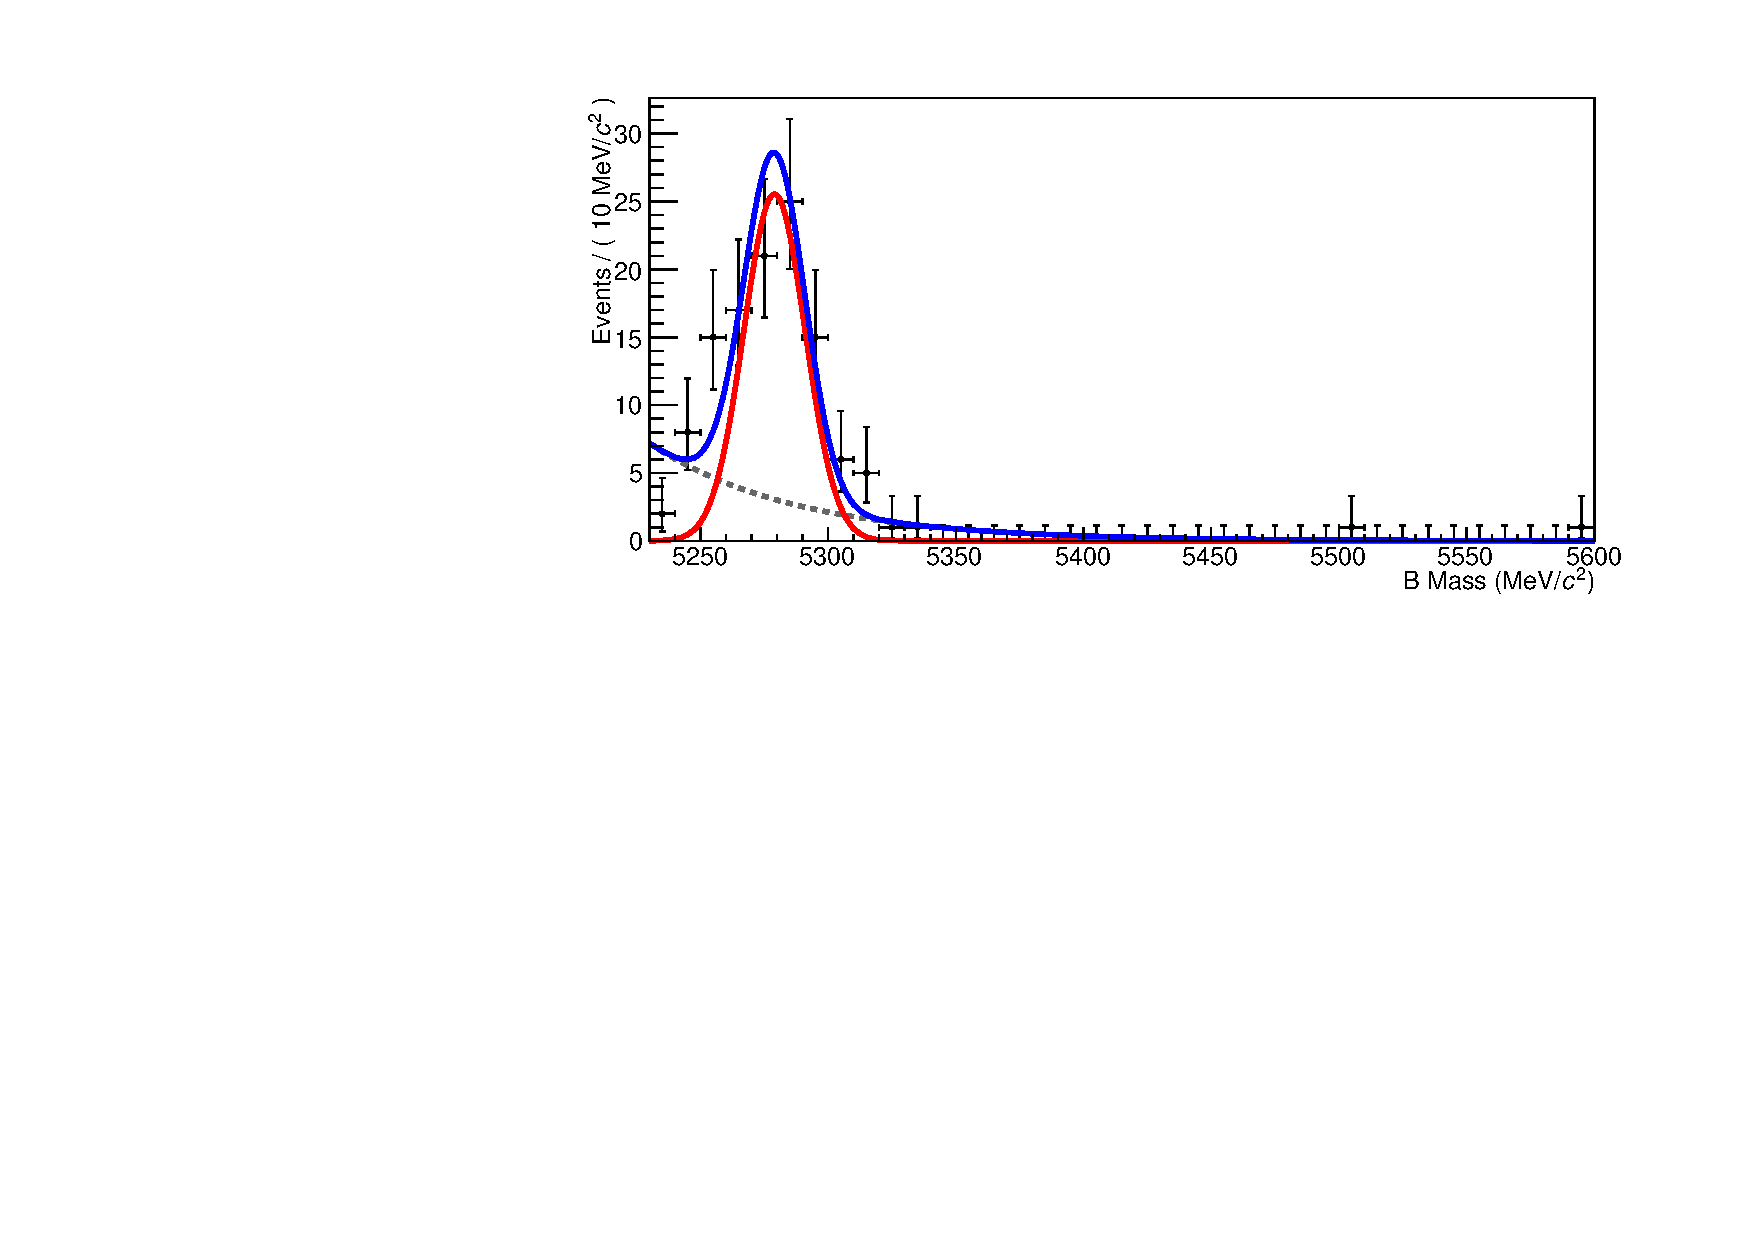
\includegraphics[width=0.7\linewidth]{figures/backgrounds/B2DpipipiFit_KPi_LL_FD0_run2.pdf}
\put(-100,100) {(a)}
\hfill
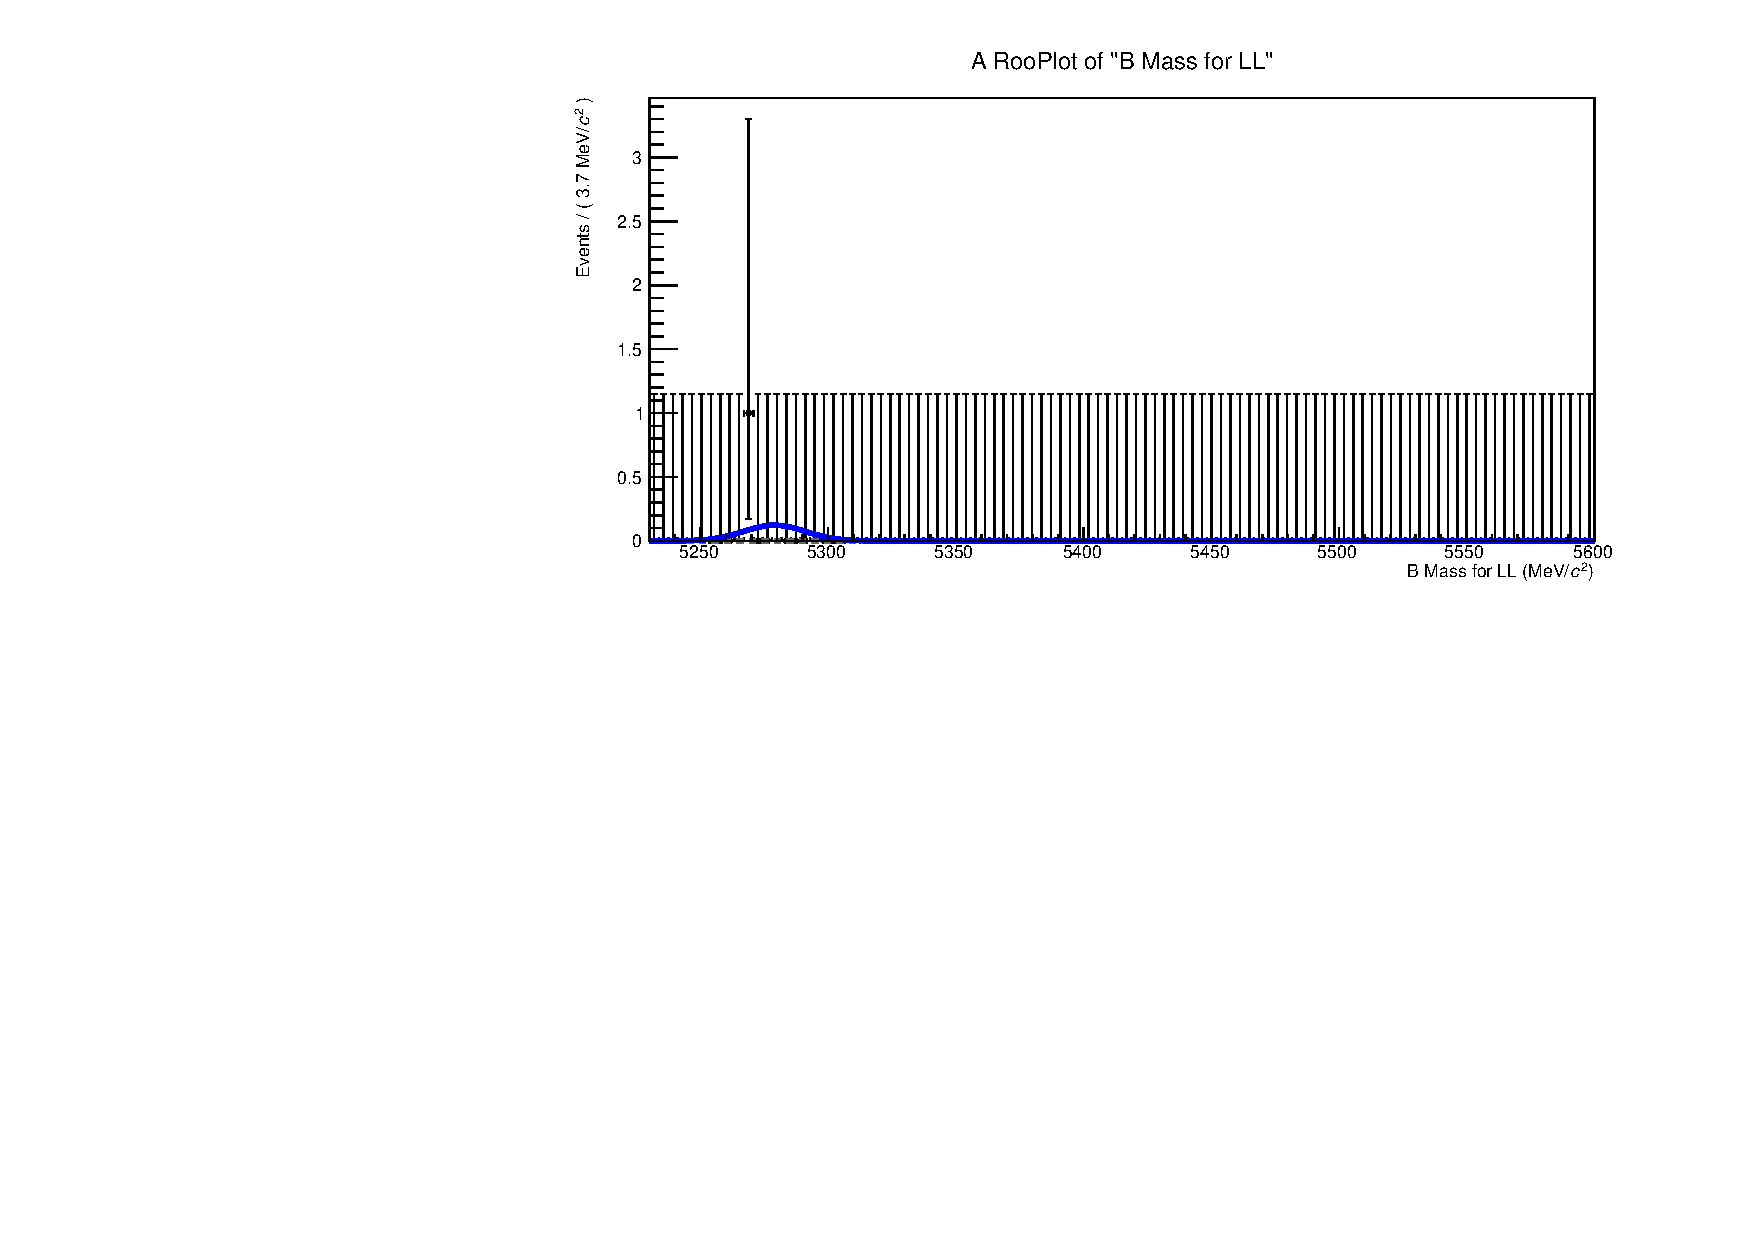
\includegraphics[width=0.7\linewidth]{figures/backgrounds/B2DpipipiFit_KPi_LL_FD5_run2.pdf}
\put(-100,100) {(b)}
\caption{Fits to the Run 2 refitted B mass taking \decay{\Dz}{\Km\pip} candidates from the \KS mass sidebands after a FD significance cut (a) greater than 0 and (b) greater than 5$\sigma$. Expected  \decay{\B}{\D\pi\pi\pi} yield in the signal region with FD significance $>$ 0 is $77 \pm 11$ and signal yield with FD significance $>$ 5 is $1.0 \pm 1.0$. A Gaussian is used to model the signal and an exponential for the combinatoric background}
\label{strangelessfits}
\end{figure}

\subsection{Non-resonant $B \to DK_s\pi$}
\label{sec:backgrounds:non-resonant}

Non-resonant background is reduced by removing events in which the \KS\pion invariant mass is greater than 75 MeV from the nominal \Kstarpm mass. \decay{\Bpm}{\D\Kstarpm} is a Scalar $\to$ Scalar Vector decay, which means the \Kstarpm must be londitudially polarised, so the $K_s$ helicity angle of pure \D\Kstarpm events follows a $\cos^2\theta$ distribution, as shown in Figure \ref{helicitycut}, compared to the uniform distribution of non-resonant components. It can be seen from Figure \ref{helicitycut} that the \KS helicity angle distribution is not symmetric, this is discussed in detail in Appendix \ref{sec:app:helicityangle}. Removing events with an absolute value of $\cos^2\theta$ less than 0.3 improves the purity of \D\Kstarpm decays compared to non-resonant background.

\begin{figure}[h]
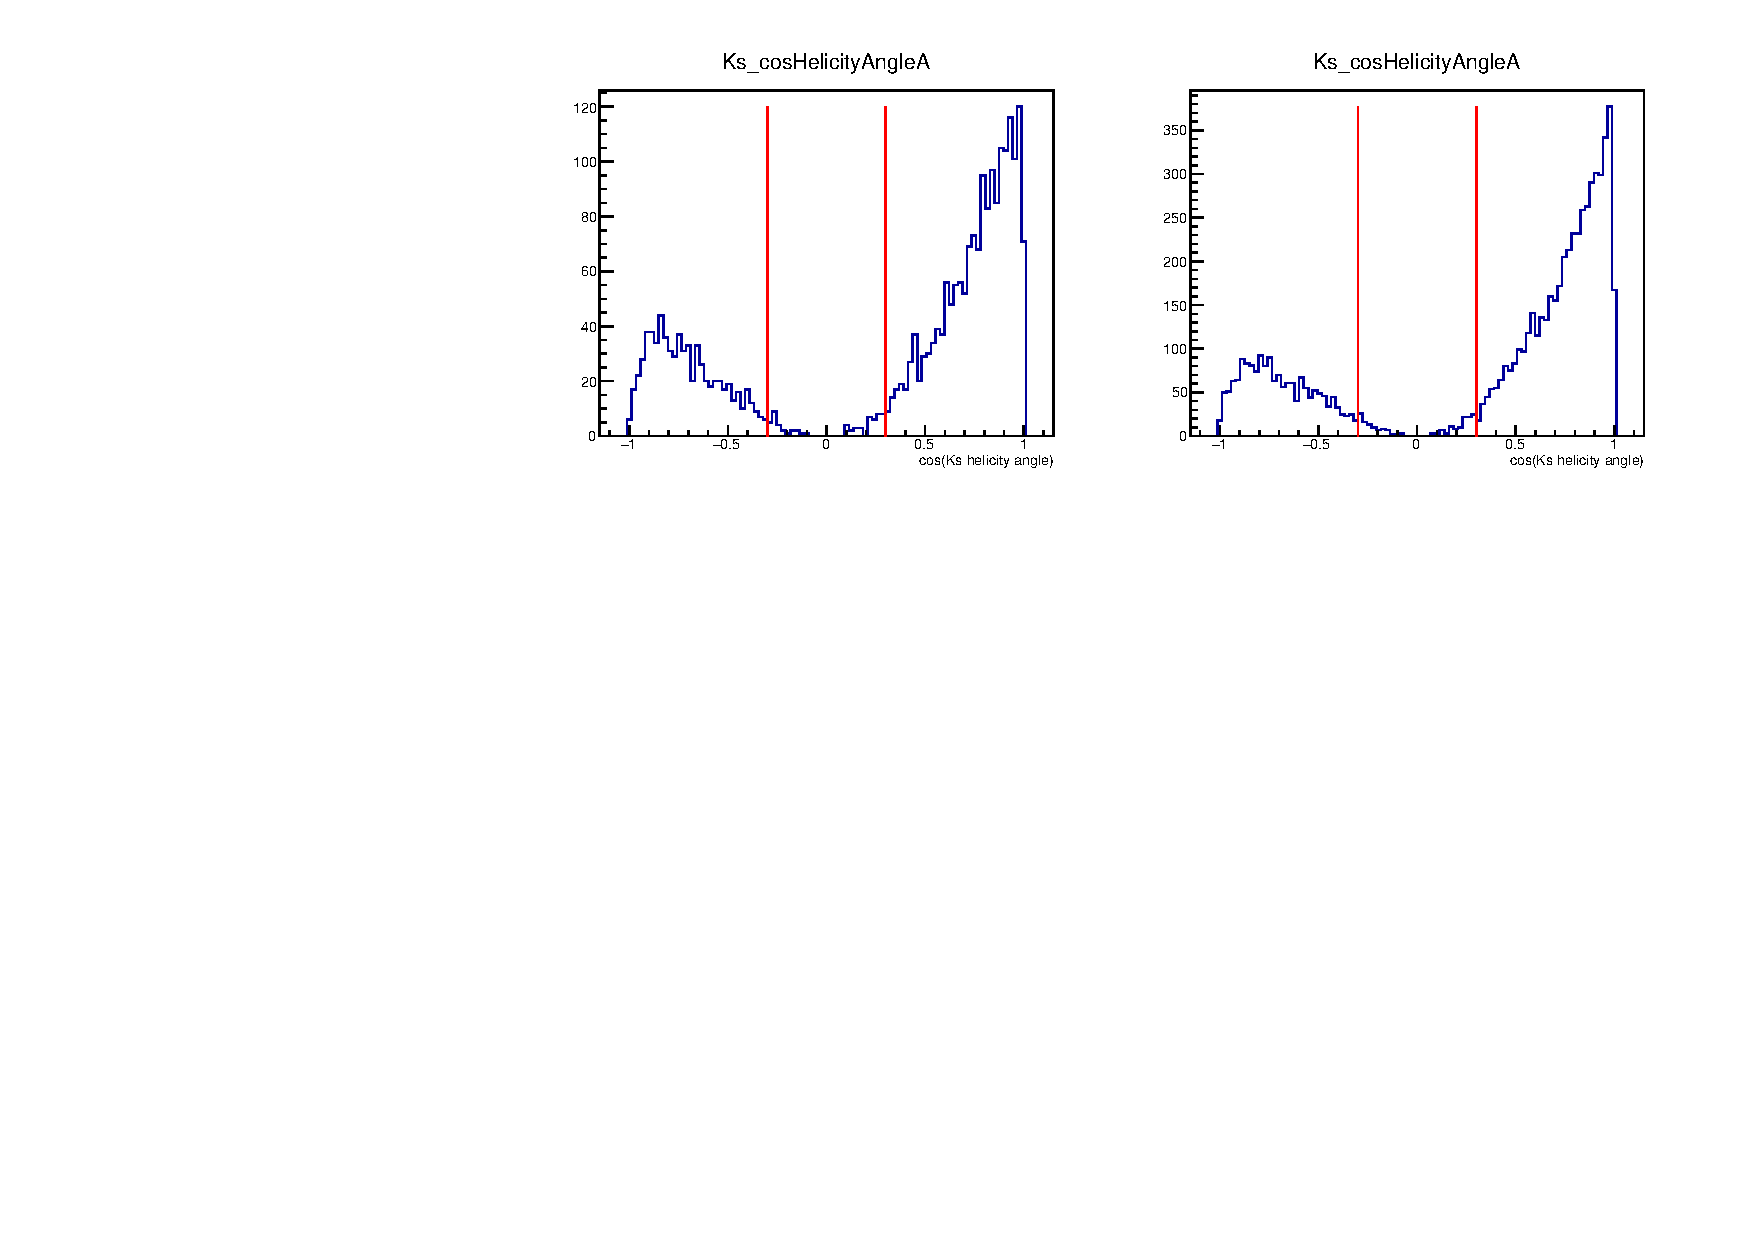
\includegraphics[width=\linewidth]{figures/backgrounds/KsHelicityCut.pdf}
\put(-400,100) {(a)}
\put(-170,100) {(b)}
\caption{MC distribution of the cosine of Ks helicity angle for (a) LL candidates and (b) DD candidates}
\label{helicitycut}
\end{figure}

It is necessary to estimate the fraction of non-resonant \decay{\B}{\D\KS\pi} in the signal candidates. Figure \ref{kshelicitycomparison} shows a comparison of \KS helicity angle and the \KS momentum between signal MC and sWeighted data. There is a discrepancy in both \KS helicity angle distribution and the \KS momentum distribution. The discrepancy in the momentum distribution was corrrected by reweighting the MC, the resulting helicity angle distribution is consistent with the data, as shown in Figure \ref{kshelicitycomparisonreweighted}.

\begin{figure}[h]
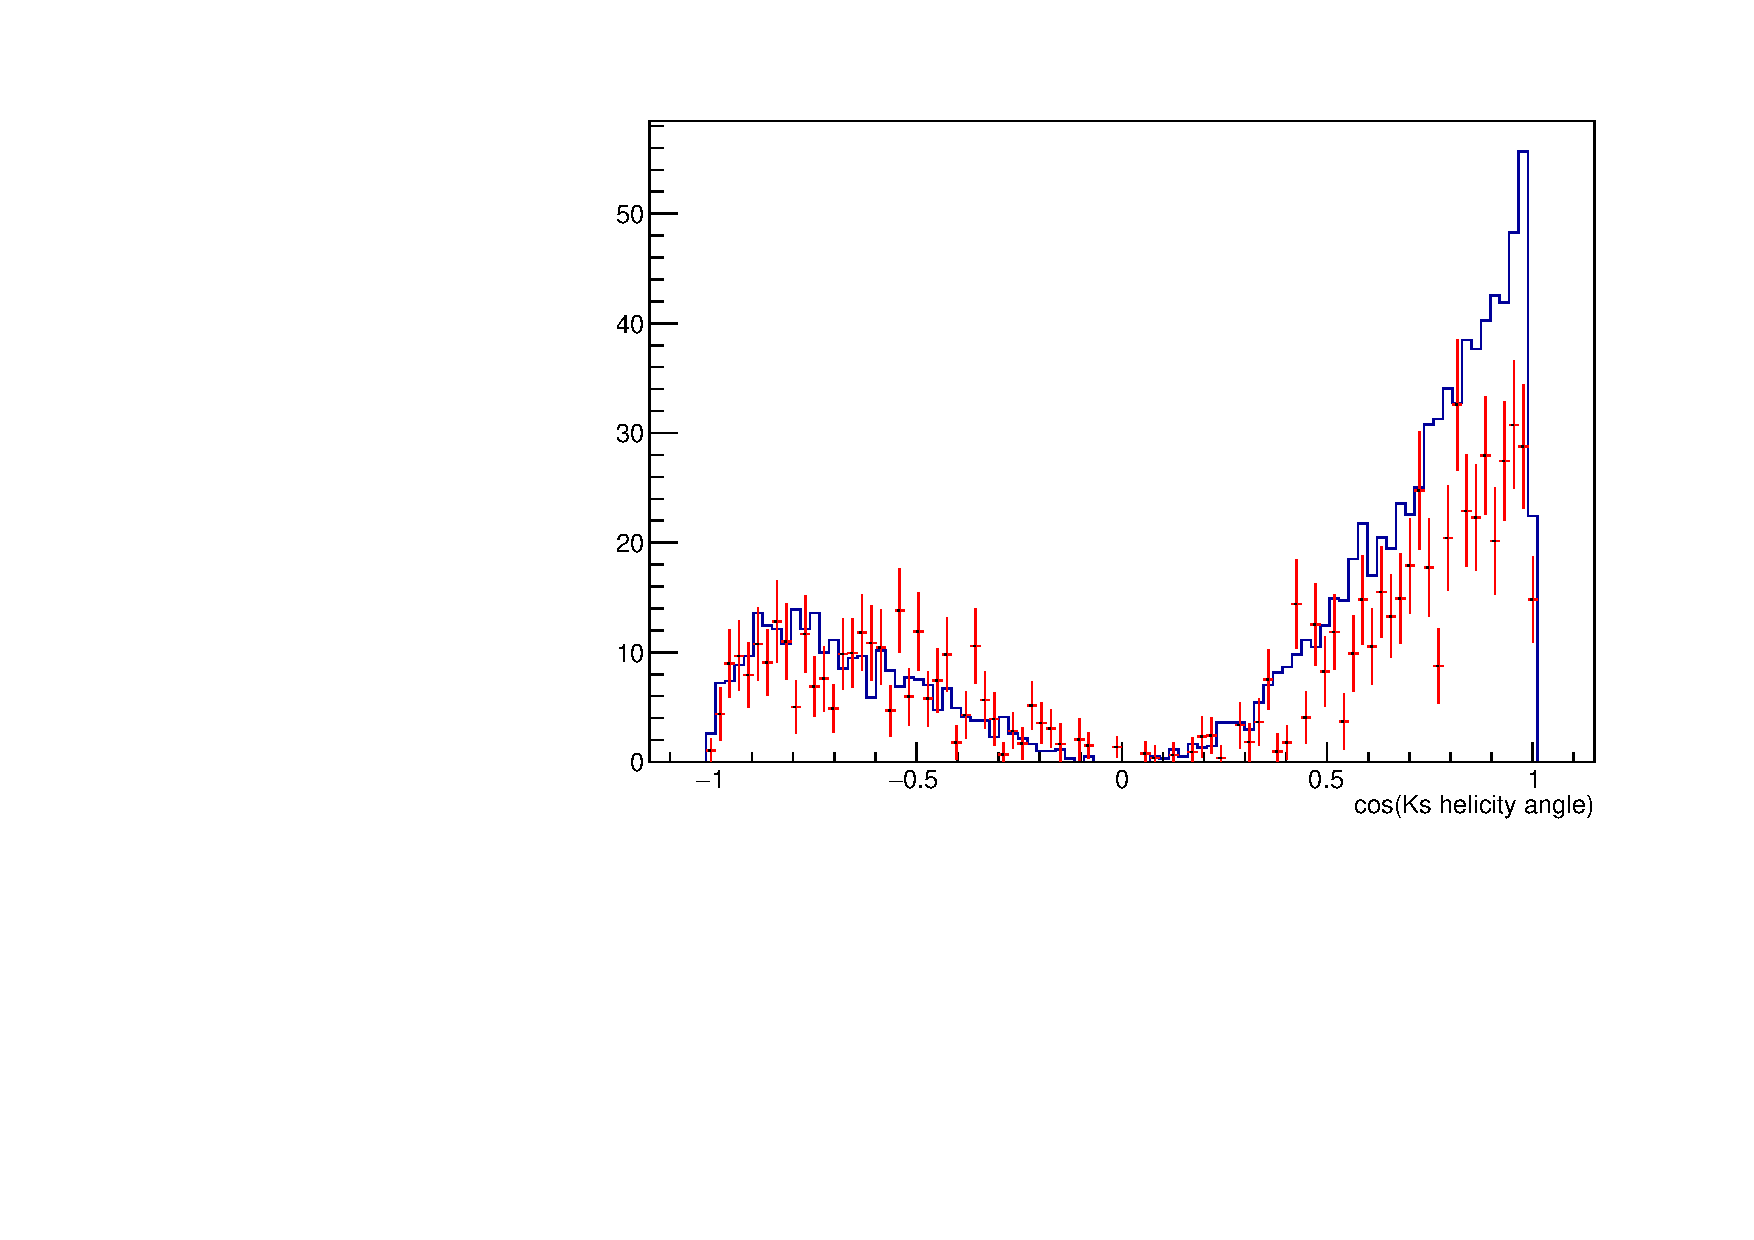
\includegraphics[width=0.5\linewidth]{figures/backgrounds/KsHelicityAngle_sweighted.pdf}
\put(-170,100) {(a)}
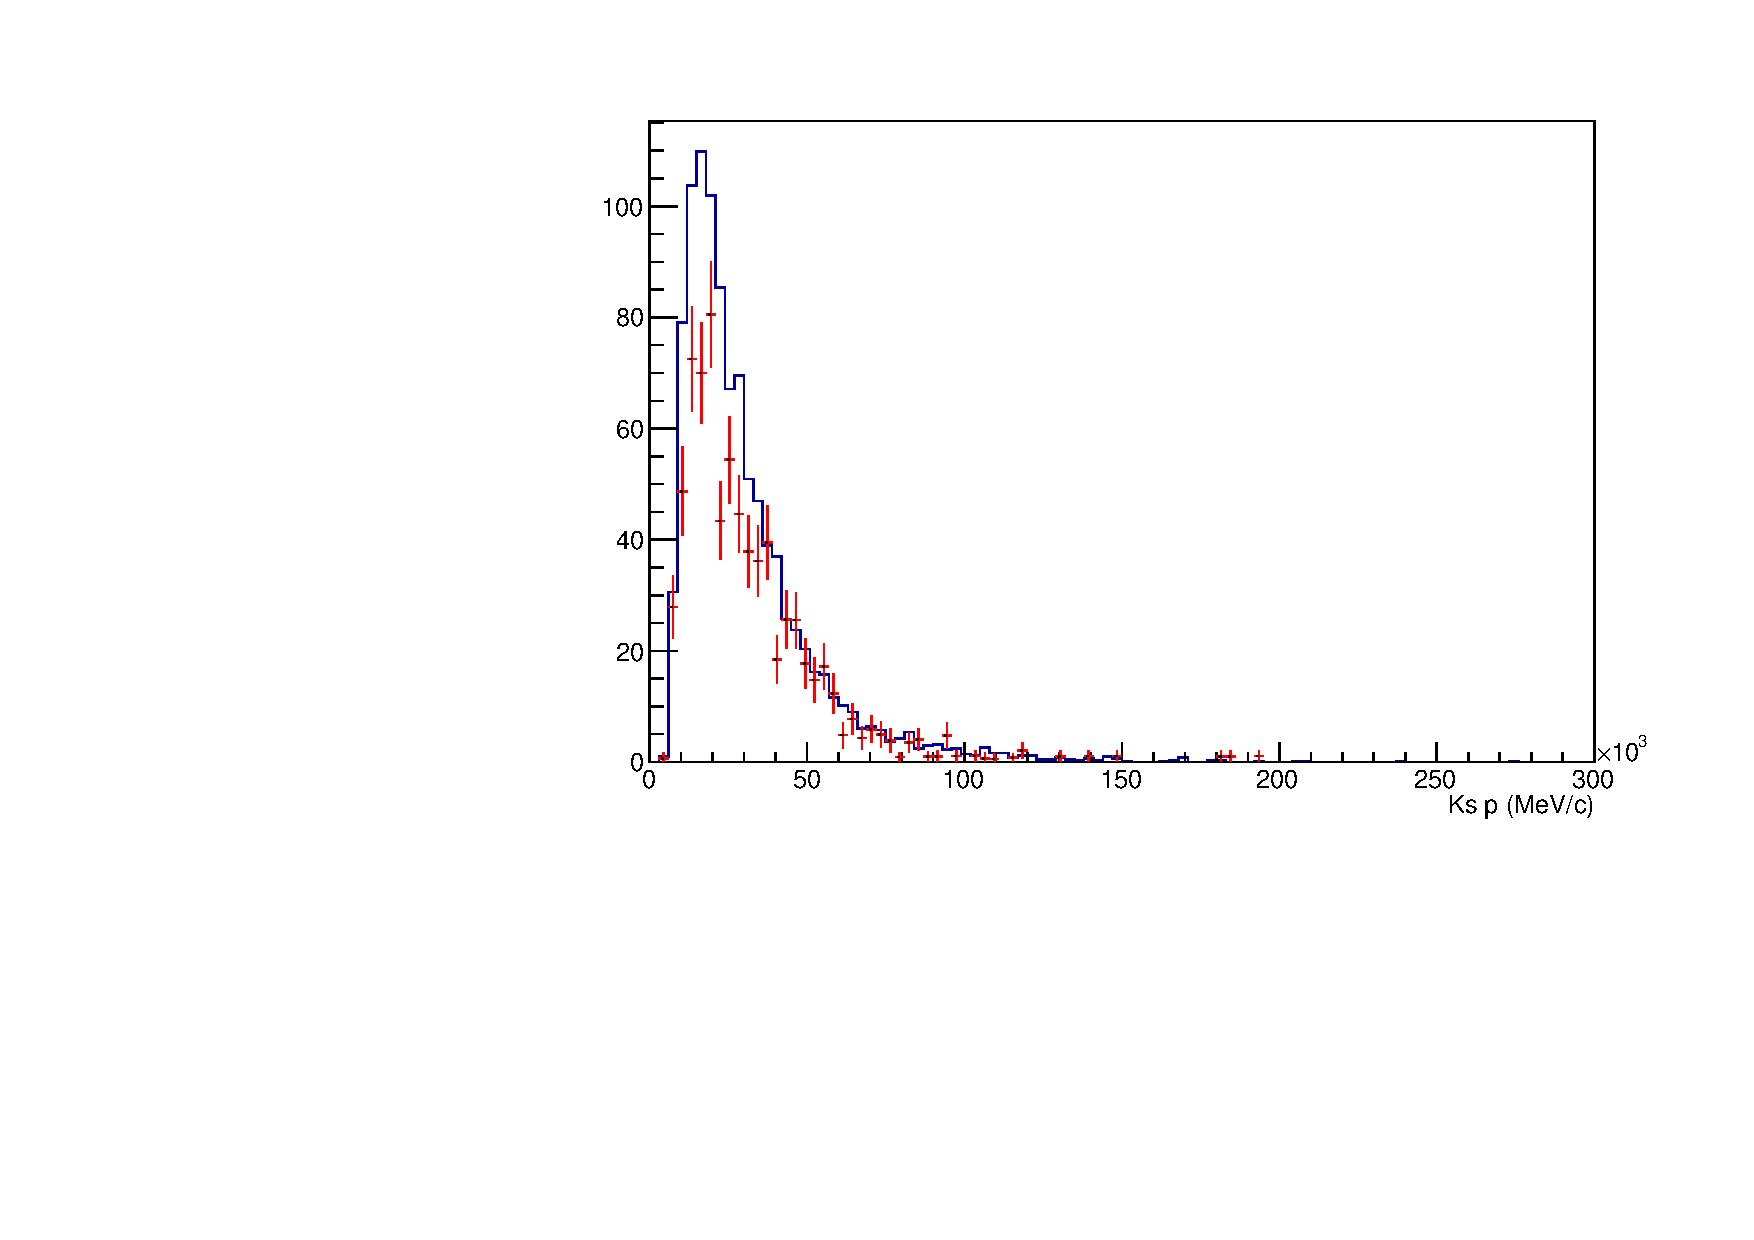
\includegraphics[width=0.5\linewidth]{figures/backgrounds/KsP_sweighted.pdf}
\put(-170,100) {(b)}
\caption{Comparison of (a) cosine of the helicity angle distribution and (b) the \KS momentum distribution in sWeighted data (red) and MC (blue)}
\label{kshelicitycomparison}
\end{figure}

\begin{figure}[h]
\centering
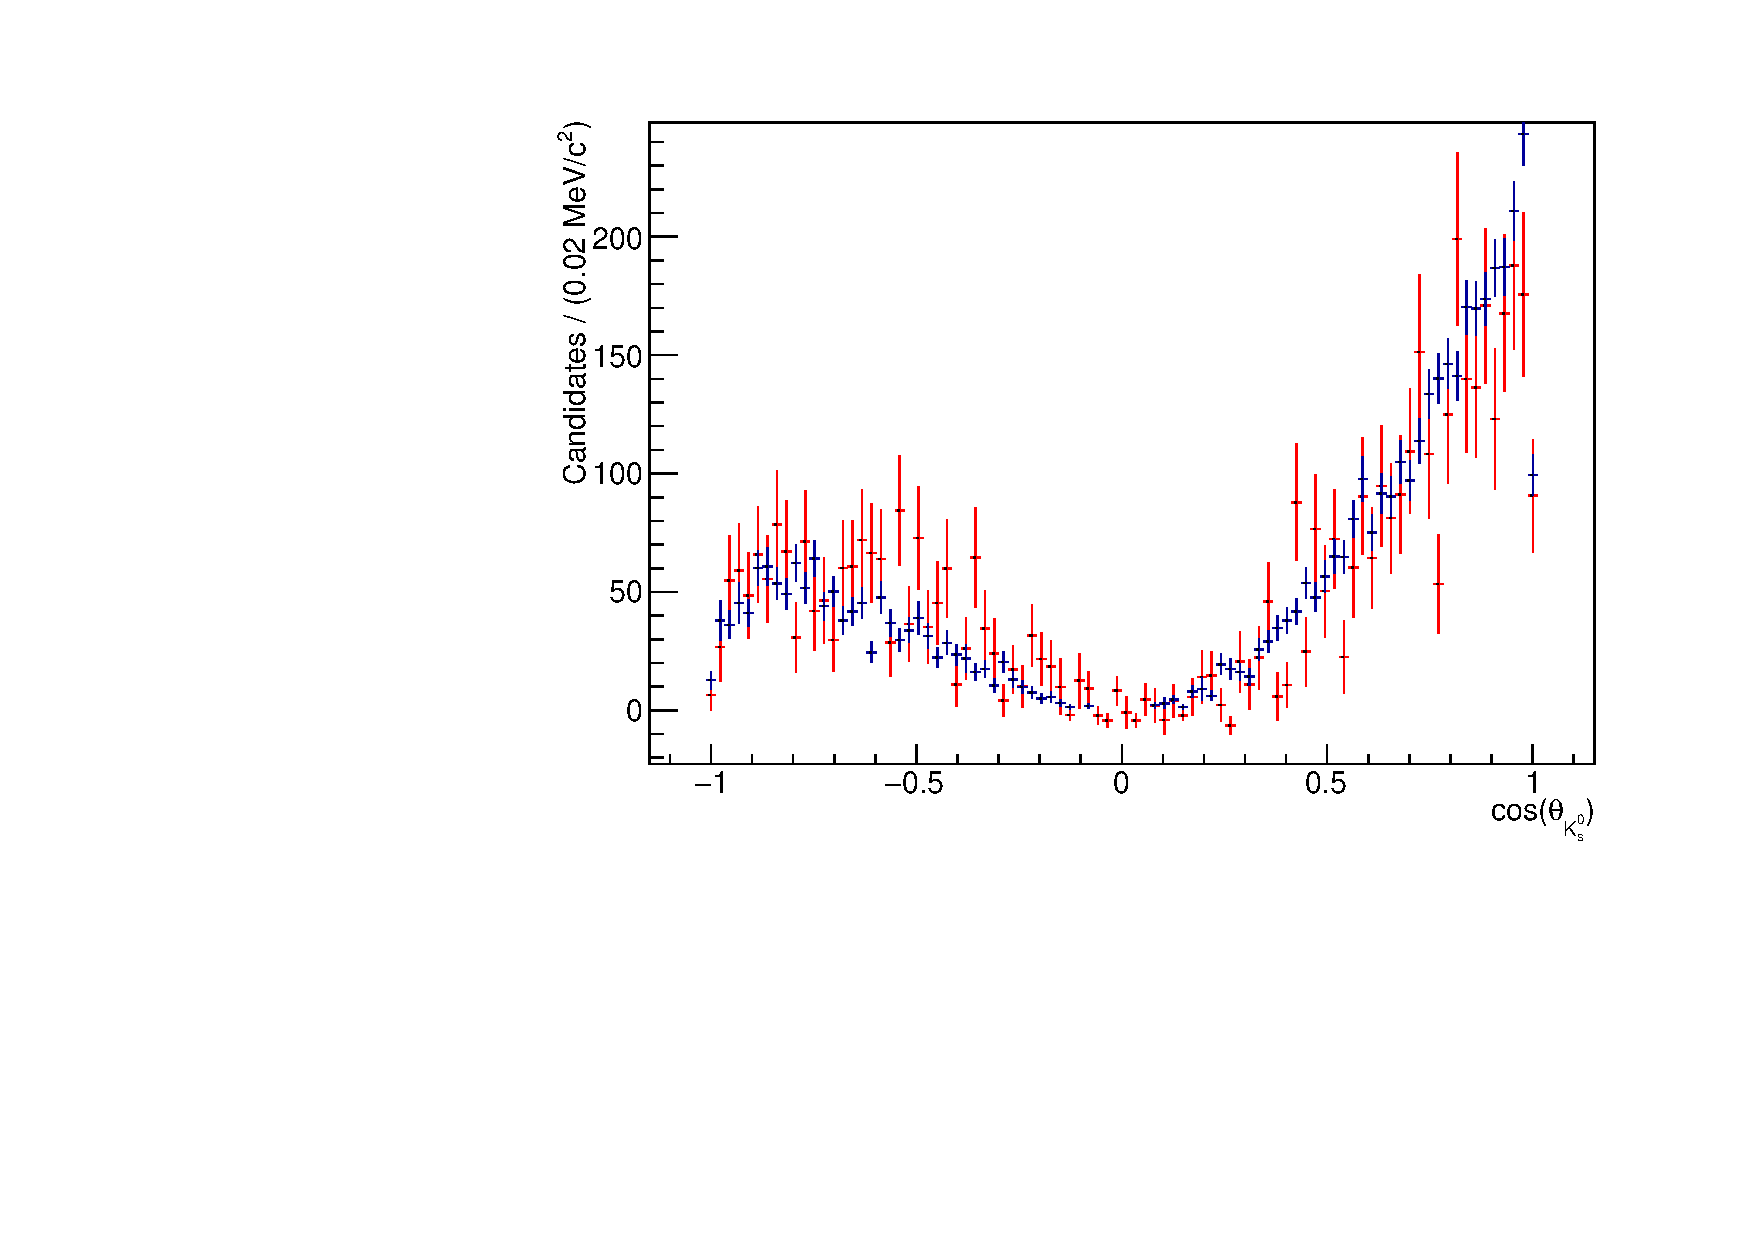
\includegraphics[width=0.6\linewidth]{figures/backgrounds/KsHelicityAngle_sweighted_MCweighted.pdf}
\caption{Comparison of cosine of the helicity angle distribution in sWeighted data (red) and MC (blue) reweighted to give the same \KS momentum distribution}
\label{kshelicitycomparisonreweighted}
\end{figure}

The parameter $\kappa$, defined in Section \ref{sec:interpretation:coherence}, is a measure of the non-$DK(892)^*$ contribution, which is expected to mainly consist of non-resonant contribution, but could include other resonances. In this analysis the value of $\kappa$ is estimated and then used alongside the \CP observables to extract \Pgamma, $r_B$ and $\delta_B$. The parameter $\kappa$ is estimated by constructing an amplitude model and generating many toys by varying the amplitudes and phases of the model components, this method is detailed in Section \ref{sec:interpretation:coherence}. The estimated value of $\kappa$ is $0.95 \pm 0.06$.

\subsection{Favoured $\to$ Supressed crossfeed}
\label{sec:backgrounds:crossfeed}

The doubly Cabibo supressed ADS mode, \decay{\Bm}{\D(\Kp\pim)\Kstarm}, can have contamination coming from the favoured \decay{\Bm}{\D(\Km\pip)\Kstarm} mode, where the daughter mass hypotheses are swapped, i.e. the kaon is misidentified as a pion and the pion is misidentified as a kaon. The favoured mode has a braching ratio 281 times higher than the ADS mode. Implementation of PID cuts of the \D daughters significantly reduces this background, however in order to reduce it to negligible levels a veto is applied. The \Dz mass is reconstructed where both daughter mass hypotheses are swapped, this is required to be greater than 15 MeV away from the nominal \Dz mass. This veto window is illustrated in Figure \ref{Dmassveto}, which shows the MC distributions for DD canidates in Run 1. The veto is only applied to the ADS mode in this analysis. It is found to be 92.5\% efficient at retaining genuine signal, corresponding to events that lie within the red lines in Figure \ref{Dmassveto} (a), while only retaining 8.7\% of double misID background, coresponding to events that lie within the red lines in Figure \ref{Dmassveto} (b). For the 4-body modes the same background can appear in the suppressed \decay{\Bm}{\D(\Kp\pim\pip\pim)\Kstarm} mode due to contamination from the favoured \decay{\Bm}{\D(\Km\pip\pim\pip)\Kstarm}. There are two \pip mesons that could be misidetified as a \Kp meson, therefore in this case two vetos need to be applied. The \Dz mass is reconstructed as a swapped mass hypothesis where the kaon is swapped with the lower momentum pion and the kaon is swapped with the higher momentum pion. The veto is applied to both these reconstructed masses as shown in Figure \ref{Dmassveto4body}.

\begin{figure}[h]
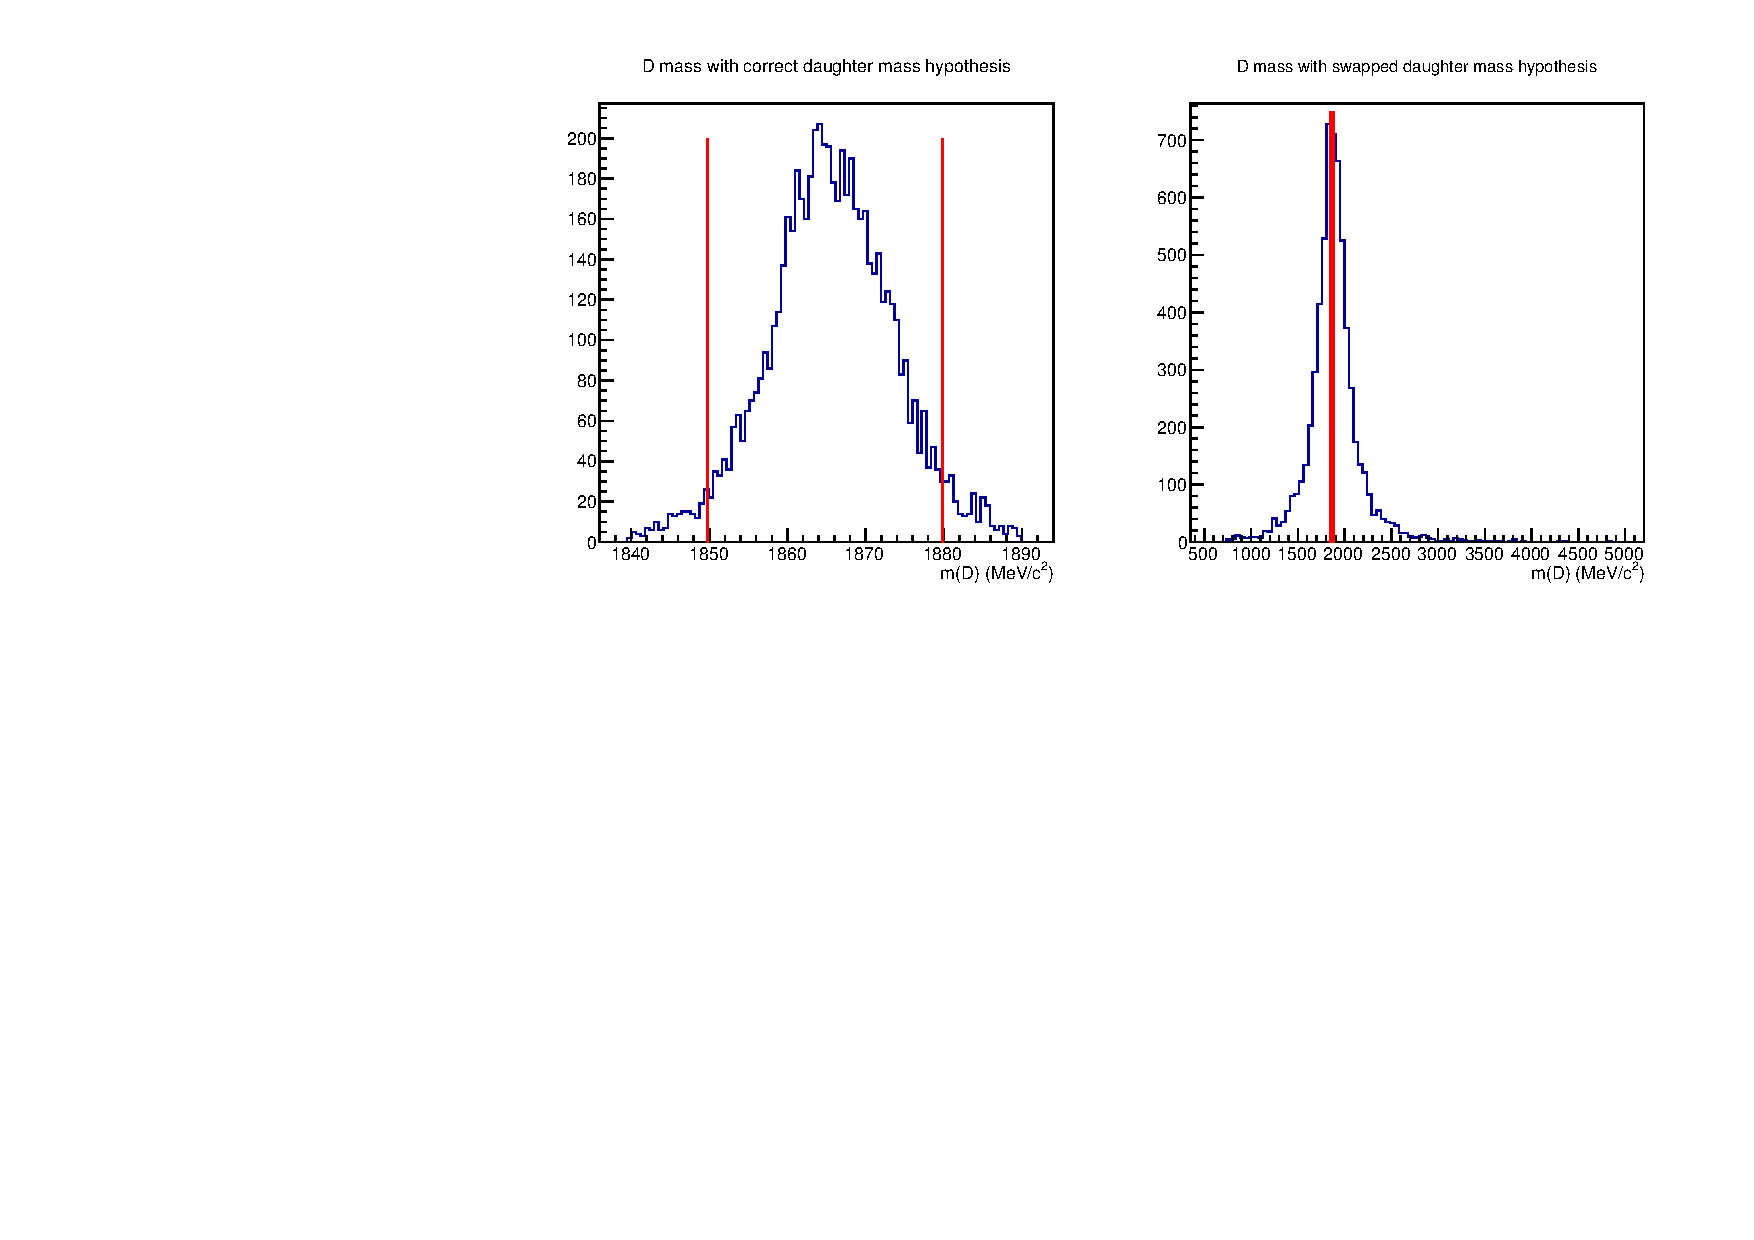
\includegraphics[width=\linewidth]{figures/backgrounds/Dmassveto.pdf}
\put(-410,150) {(a)}
\put(-180,150) {(b)}
\caption{MC distributions for DD canidates in Run 1 showing D mass with (a) the correct D daughter mass hypothesis and (b) the swapped D daughter mass hypothesis. The red lines correcpond to the double misID veto selection window applied to the ADS mode}
\label{Dmassveto}
\end{figure}

\begin{figure}[h]
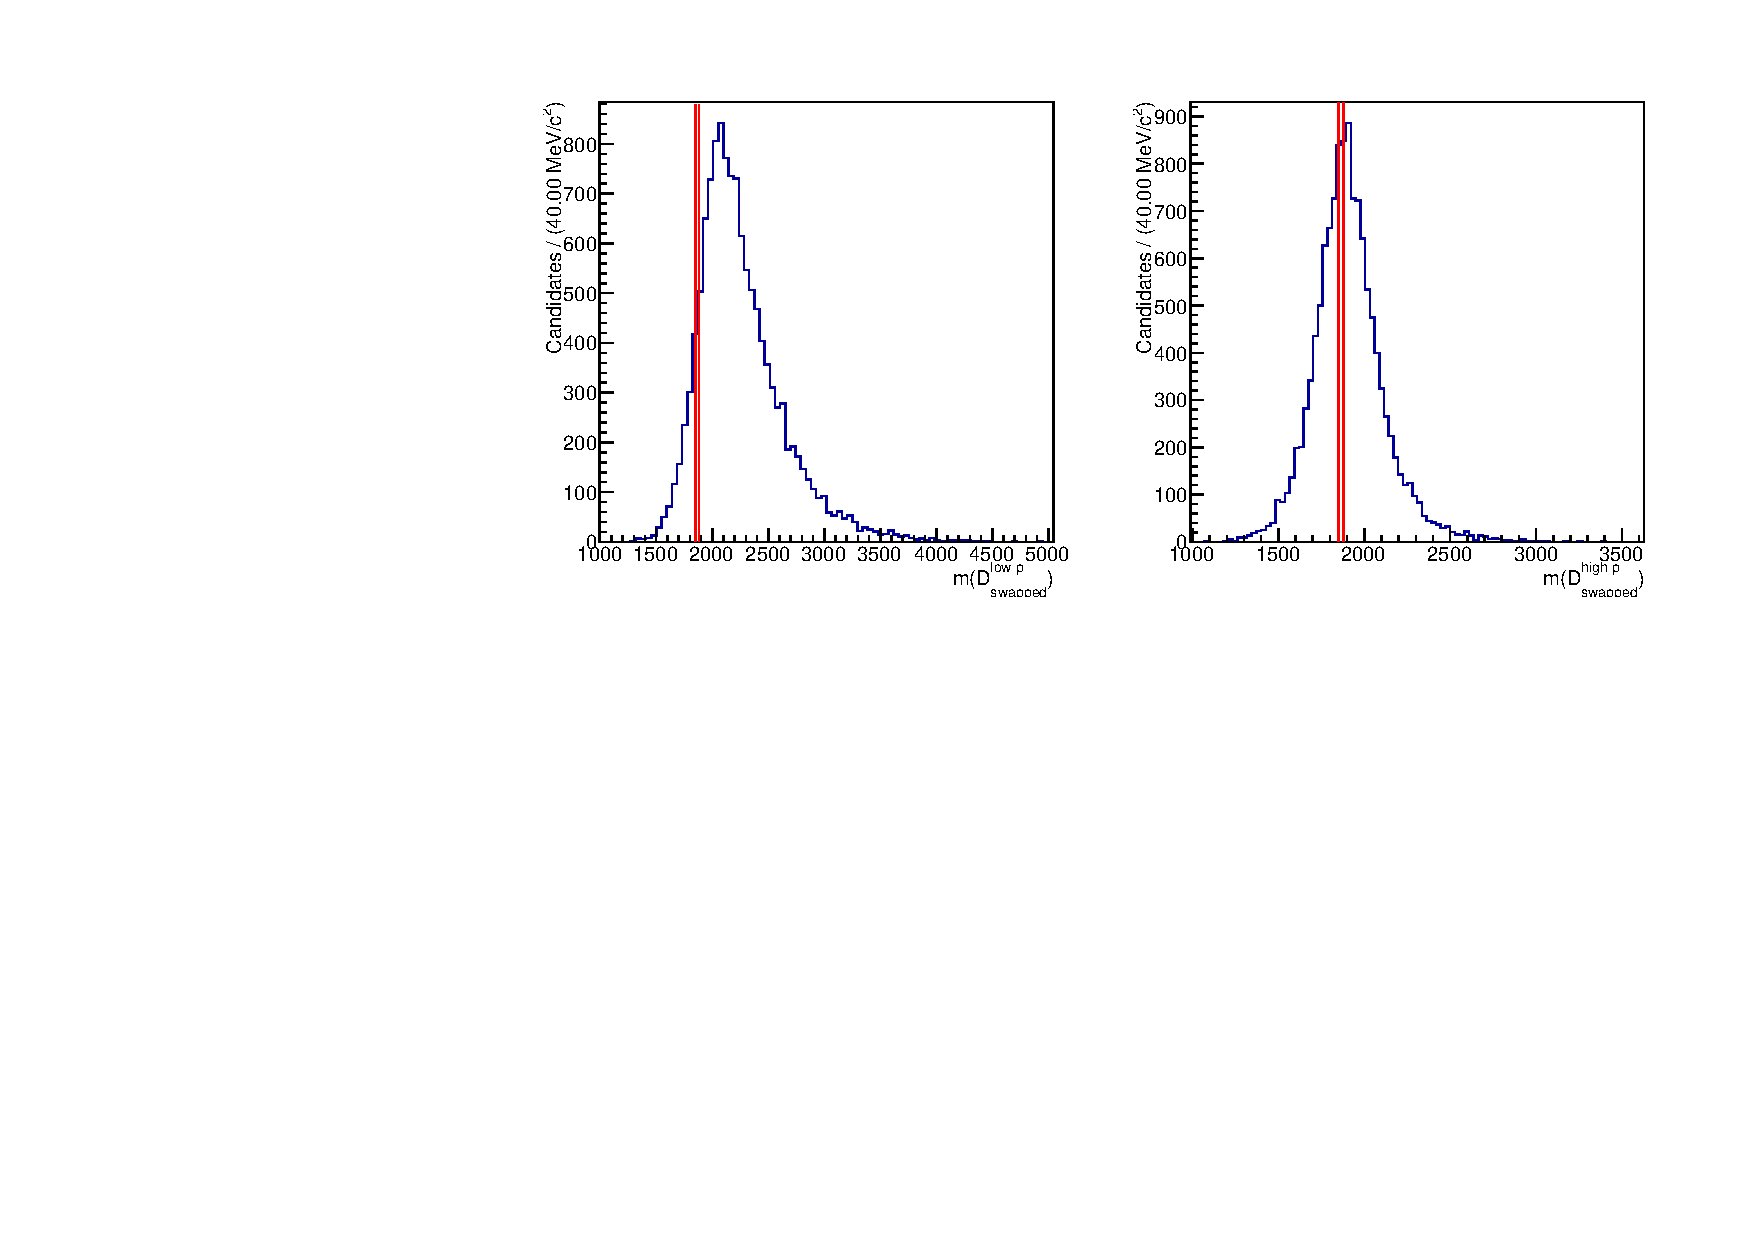
\includegraphics[width=\linewidth]{figures/backgrounds/Dmassveto_4body.pdf}
\put(-410,150) {(a)}
\put(-180,150) {(b)}
\caption{MC distributions for DD canidates in Run 2 showing the swapped D daughter mass hypothesis where (a) the kaon is swapped with the lower momentum pion and (b) the kaon is swapped with the higher momentum pion. The red lines correspond to the double misID veto selection window applied to the suppressed mode}
\label{Dmassveto4body}
\end{figure}

In order to determine the overall crossfeed contamination in the supressed mode the efficiency of the D mass window, double misID veto and PID requirements are taken into account for both the normal and swapped \Dz mass hypothesis. For the 2-body mode, these efficiencies are listed in Tables \ref{crossfeedefficienciesRun1} and \ref{crossfeedefficienciesRun2}. The proportion of events that will enter the supressed mode fit relative to the total \decay{\Bm}{\D(\Kp\pim)\Kstarm} is estimated to be $9.5 \times 10^{-3}$ for LL and $6.5 \times 10^{-3}$ for DD in Run 1, and $5.6 \times 10^{-3}$ for LL and $5.3 \times 10^{-3}$ in Run 2. Similarly for the 4-body mode, the efficiencies are listed in Tables \ref{crossfeedefficienciesk3piRun1} and \ref{crossfeedefficienciesk3piRun2}. The proportion of events that will enter the supressed mode fit relative to the total \decay{\Bm}{\D(\Kp\pim\pip\pim)\Kstarm} is estimated to be $2.7 \times 10^{-3}$ for LL and $1.0 \times 10^{-3}$ for DD in Run 1, and $1.4 \times 10^{-3}$ for LL and $6.3 \times 10^{-4}$ in Run 2. Therefore, the contribtuion of the crossfeed in the supressed mode is negligible.

%The tighter BDT cut applied in the ADS mode for DD candidates also has to be taken into account. The relative BDT efficiency is 0.877 for Run 1 and 0.902 for Run 2.

\begin{table}[h]
\centering
\begin{tabular}{ccc}
\hline
Selection cut & $[K_K^-\pi_\pi^+]_D$ efficiency & $[K_\pi^-\pi_K^+]_D$ efficiency \\
\hline
\Dz window: $\pm$ 25 MeV & 0.961 $\pm$ 0.003 & 0.116 $\pm$ 0.005 \\
Crossfeed veto $\pm$ 15 MeV & 0.930 $\pm$ 0.004 & 0.122 $\pm$ 0.014 \\
PID selection & 0.734 $\pm$ 0.002 & 0.00158 $\pm$ 0.00002 \\
\hline
Total & 0.655 $\pm$ 0.004 & (2.2 $\pm$ 0.3) $\times 10^{-5}$ \\
\hline
\end{tabular}
\begin{tabular}{ccc}
\hline
Selection cut & $[K_K^-\pi_\pi^+]_D$ efficiency & $[K_\pi^-\pi_K^+]_D$ efficiency \\
\hline
\Dz window: $\pm$ 25 MeV & 0.961 $\pm$ 0.002 & 0.123 $\pm$ 0.003 \\
Crossfeed veto $\pm$ 15 MeV & 0.925 $\pm$ 0.002 & 0.087 $\pm$ 0.007 \\
PID selection & 0.747 $\pm$ 0.002 & 0.00144 $\pm$ 0.00005 \\
\hline
Total & 0.663 $\pm$ 0.003 & (1.53 $\pm$ 0.14) $\times 10^{-5}$ \\
\hline
\end{tabular}
\caption{Efficiencies of the \Dz mass window, crossfeed veto and \Dz daughter PID cuts for \decay{\Bpm}{[\Kmp\pipm]_D\Kstarpm} events in Run 1. The first table shows the LL efficiencies and the second shows the DD efficiencies. The proprtion of crossfeed events from favoured \decay{\Bpm}{[\Kpm\pimp]_D\Kstarpm} mode which are expected in \decay{\Bpm}{[\Kmp\pipm]_D\Kstarpm} mode fit is $(9.5 \pm 1.2) \times 10^{-3}$ for LL and $(6.5 \pm 0.6) \times 10^{-3}$ for DD}
\label{crossfeedefficienciesRun1}
\end{table}

\begin{table}
\centering
\begin{tabular}{ccc}
\hline
Selection cut & $[K_K^-\pi_\pi^+]_D$ efficiency & $[K_\pi^-\pi_K^+]_D$ efficiency \\
\hline
\Dz window: $\pm$ 25 MeV & 0.954 $\pm$ 0.002 & 0.118 $\pm$ 0.003 \\
Crossfeed veto $\pm$ 15 MeV & 0.929 $\pm$ 0.003 & 0.108 $\pm$ 0.009 \\
PID selection & 0.811 $\pm$ 0.002 & 0.00112 $\pm$ 0.00002 \\
\hline
Total & 0.719 $\pm$ 0.003 & (1.43 $\pm$ 0.12) $\times 10^{-5}$ \\
\hline
\end{tabular}
\begin{tabular}{ccc}
\hline
Selection cut & $[K_K^-\pi_\pi^+]_D$ efficiency & $[K_\pi^-\pi_K^+]_D$ efficiency \\
\hline
\Dz window: $\pm$ 25 MeV & 0.9553 $\pm$ 0.0012 & 0.1181 $\pm$ 0.0019 \\
Crossfeed veto $\pm$ 15 MeV & 0.9284 $\pm$ 0.0016 & 0.111 $\pm$ 0.005 \\
PID selection & 0.821 $\pm$ 0.002 & 0.00104 $\pm$ 0.00002 \\
\hline
Total & 0.728 $\pm$ 0.002 & (1.37 $\pm$ 0.08) $\times 10^{-5}$ \\
\hline
\end{tabular}
\caption{Efficiencies of the \Dz mass window, crossfeed veto and \Dz daughter PID cuts for \decay{\Bpm}{[\Kmp\pipm]_D\Kstarpm} events in Run 2. The first table shows the LL efficiencies and the second shows the DD efficiencies. The proprtion of crossfeed events from favoured \decay{\Bpm}{[\Kpm\pimp]_D\Kstarpm} mode which are expected in \decay{\Bpm}{[\Kmp\pipm]_D\Kstarpm} mode fit is $(5.6 \pm 0.5) \times 10^{-3}$ for LL and $(5.3 \pm 0.3) \times 10^{-3}$ for DD}
\label{crossfeedefficienciesRun2}
\end{table}

\begin{table}[h]
\centering
\begin{tabular}{ccc}
\hline
Selection cut & $[K_K^-\pi_\pi^+\pim\pip]_D$ efficiency & $[K_\pi^-\pi_K^+\pim\pip]_D$ efficiency \\
\hline
\Dz window: $\pm$ 25 MeV & 0.749 $\pm$ 0.011 & 0.009 $\pm$ 0.002 \\
Crossfeed veto $\pm$ 15 MeV & 0.907 $\pm$ 0.008 & 0.50 $\pm$ 0.13 \\
PID selection & 0.630 $\pm$ 0.002 & 0.00089 $\pm$ 0.00002 \\
\hline
Total & 0.428 $\pm$ 0.007 & (3.8 $\pm$ 1.4) $\times 10^{-6}$ \\
\hline
\end{tabular}
\begin{tabular}{ccc}
\hline
Selection cut & $[K_K^-\pi_\pi^+\pim\pip]_D$ efficiency & $[K_\pi^-\pi_K^+\pim\pip]_D$ efficiency \\
\hline
\Dz window: $\pm$ 25 MeV & 0.817 $\pm$ 0.006 & 0.0080 $\pm$ 0.0013 \\
Crossfeed veto $\pm$ 15 MeV & 0.904 $\pm$ 0.005 & 0.23 $\pm$ 0.07 \\
PID selection & 0.636 $\pm$ 0.002 & 0.00084 $\pm$ 0.00002 \\
\hline
Total & 0.470 $\pm$ 0.004 & (1.54 $\pm$ 0.5) $\times 10^{-6}$ \\
\hline
\end{tabular}
\caption{Efficiencies of the \Dz mass window, crossfeed veto and \Dz daughter PID cuts for \decay{\Bpm}{[\Kmp\pipm\pimp\pipm]_D\Kstarpm} events in Run 1. The first table shows the LL efficiencies and the second shows the DD efficiencies. The proprtion of crossfeed events from favoured \decay{\Bpm}{[\Kpm\pimp\pipm\pimp]_D\Kstarpm} mode which are expected in \decay{\Bpm}{[\Kmp\pipm\pimp\pipm]_D\Kstarpm} mode fit is $(2.7 \pm 1.0) \times 10^{-3}$ for LL and $(1.0 \pm 0.4) \times 10^{-3}$ for DD}
\label{crossfeedefficienciesk3piRun1}
\end{table}

\begin{table}
\centering
\begin{tabular}{ccc}
\hline
Selection cut & $[K_K^-\pi_\pi^+\pim\pip]_D$ efficiency & $[K_\pi^-\pi_K^+\pim\pip]_D$ efficiency \\
\hline
\Dz window: $\pm$ 25 MeV & 0.791 $\pm$ 0.003 & 0.0072 $\pm$ 0.0007 \\
Crossfeed veto $\pm$ 15 MeV & 0.905 $\pm$ 0.003 & 0.31 $\pm$ 0.05 \\
PID selection & 0.784 $\pm$ 0.002 & 0.00115 $\pm$ 0.00002 \\
\hline
Total & 0.561 $\pm$ 0.003 & (2.6 $\pm$ 0.5) $\times 10^{-6}$ \\
\hline
\end{tabular}
\begin{tabular}{ccc}
\hline
Selection cut & $[K_K^-\pi_\pi^+\pim\pip]_D$ efficiency & $[K_\pi^-\pi_K^+\pim\pip]_D$ efficiency \\
\hline
\Dz window: $\pm$ 25 MeV & 0.820 $\pm$ 0.002 & 0.0057 $\pm$ 0.0004 \\
Crossfeed veto $\pm$ 15 MeV & 0.9040 $\pm$ 0.0018 & 0.20 $\pm$ 0.03\\
PID selection & 0.798 $\pm$ 0.002 & 0.00106 $\pm$ 0.00002 \\
\hline
Total & 0.592 $\pm$ 0.002 & (1.2 $\pm$ 0.2) $\times 10^{-6}$ \\
\hline
\end{tabular}
\caption{Efficiencies of the \Dz mass window, crossfeed veto and \Dz daughter PID cuts for \decay{\Bpm}{[\Kmp\pipm\pimp\pipm]_D\Kstarpm} events in Run 2. The first table shows the LL efficiencies and the second shows the DD efficiencies. The proprtion of crossfeed events from favoured \decay{\Bpm}{[\Kpm\pimp\pipm\pimp]_D\Kstarpm} mode which are expected in \decay{\Bpm}{[\Kmp\pipm\pimp\pipm]_D\Kstarpm} mode fit is $(1.4 \pm 0.3) \times 10^{-3}$ for LL and $(6.3 \pm 1.1) \times 10^{-4}$ for DD}
\label{crossfeedefficienciesk3piRun2}
\end{table}

\clearpage

\subsection{Lambda contamination}
\label{sec:backgrounds:contamination}

The \decay{\KS}{\pip\pim} decay could have contamination coming from \decay{\Lz}{\proton\pim}, where the proton is reconstructed as a pion. It is not possible to determine possible \Lz contamination from the \KS invariant mass spectrum, where one of the \KS daughters is assigned the proton mass, because a peak at the \Lz mass cannot be distinguished from the variation near the low mass threshold. In order to distinguish between \KS decays and \Lz contamination the Armenteros-Podolanski (AP) plot is used~\cite{APplot}. The transverse momentum of the daughters with respect to the mother particle, $p_T$, is plotted against the longitudinal momentum asymmetry, which is defined as,

\begin{equation}
\frac{p_L^+ - p_L^-}{p_L^+ + p_L^-}
\end{equation}

where $p_L^{\pm}$ is the longitudinal momentum of the daughter particles with respect to the direction of the mother. The resulting AP plots for both data and MC are shown in Figure \ref{applots}. Both the data and MC samples have passed the full selection, except the MC sample does not have any PID applied. The decay products of the \decay{\KS}{\pip\pim} decay have the same mass and therefore on average their momenta is symmetrically distributed, resulting in the distribution observed in Figure \ref{applots}; these curves are the same shape as the expected distribution for a sample of pure \KS mesons. The distribution of the events in the data sample can be seen more clearly in Figure \ref{applotsdata}. Whereas for the \decay{\Lz}{\proton\pim}, the proton would, on average, take a larger proportion of the momentum resulting in an asymmteric distribution. Contamination from \Lz baryons would be clearly seen as a distinct structure on the AP plot, as illustrated in Figure \ref{apexample}. Therefore, Figure \ref{applots} shows that there is no contamination from \decay{\Lz}{\proton\pim} decays in this sample.

\begin{figure}[h]
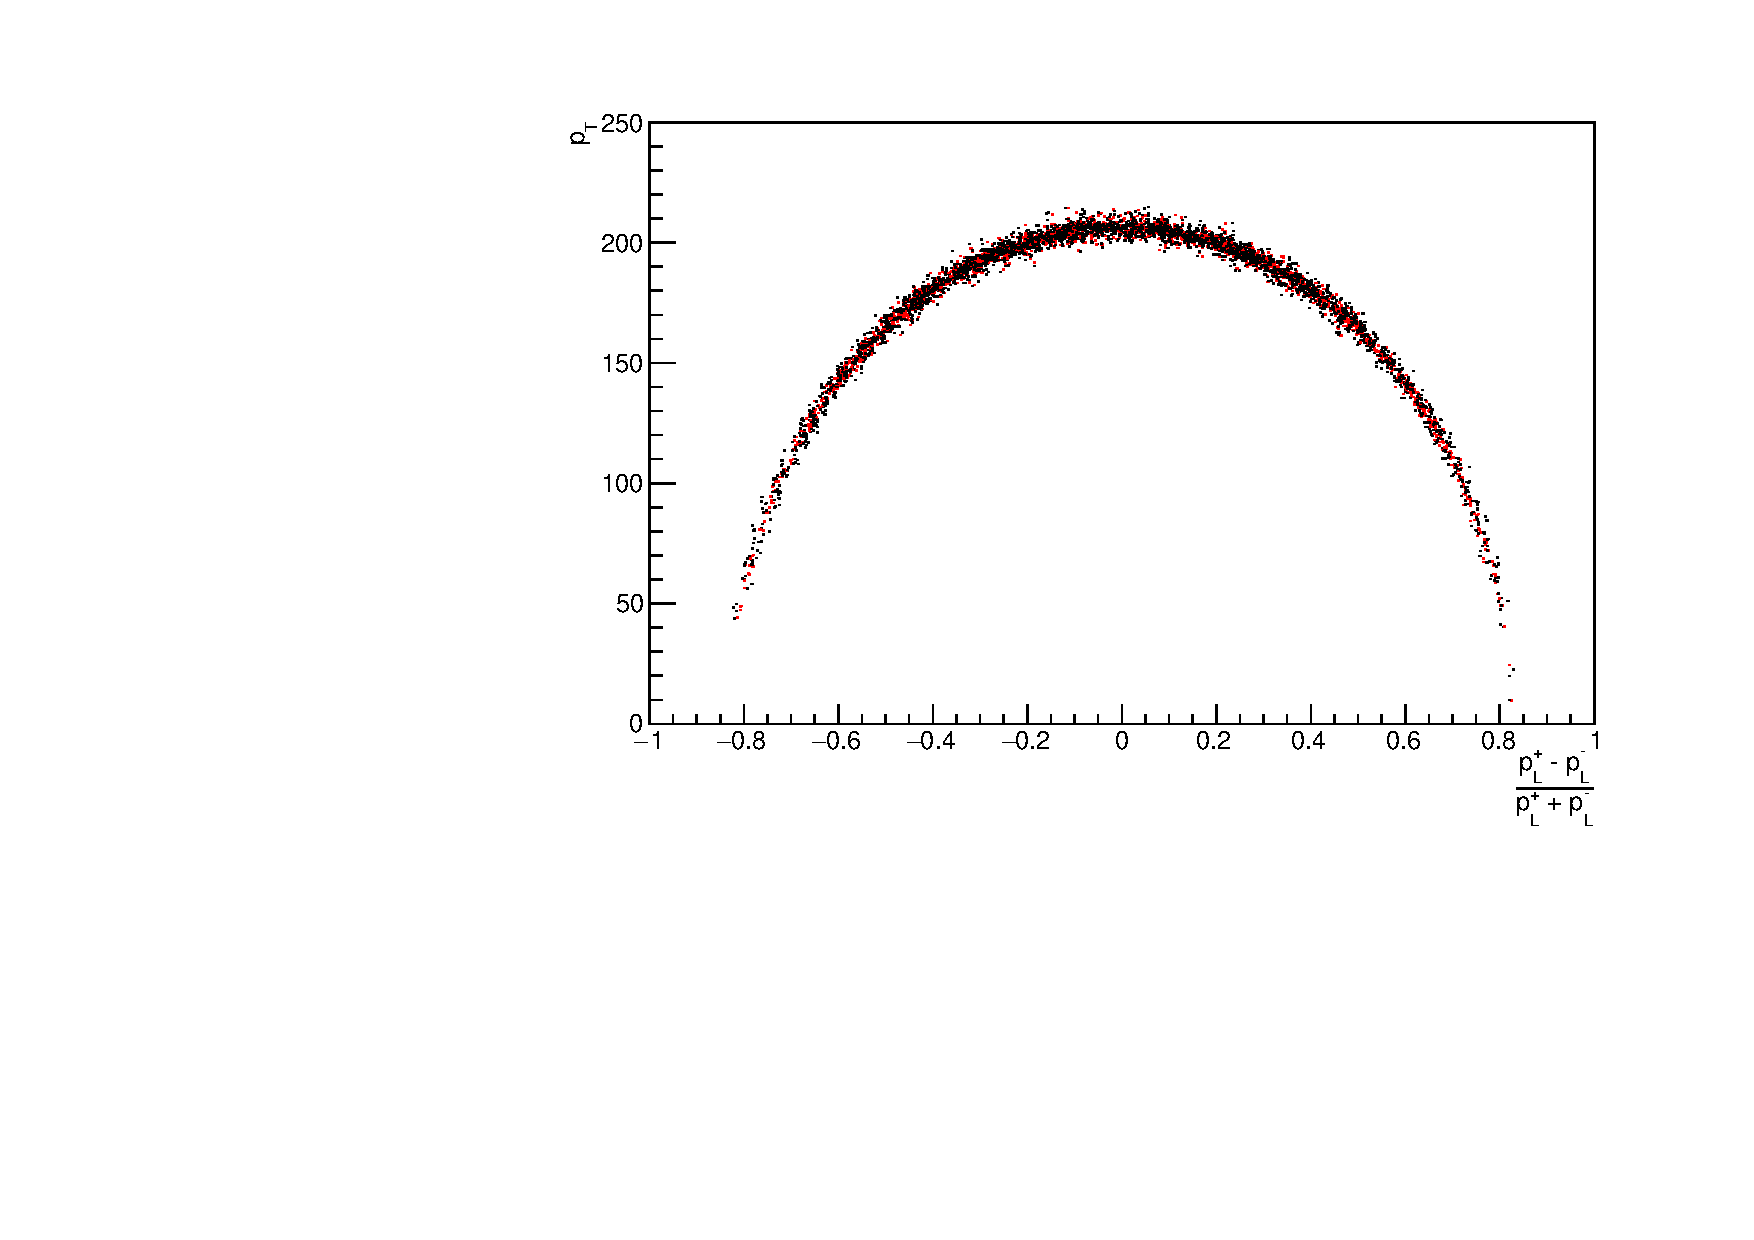
\includegraphics[width=0.5\linewidth]{figures/backgrounds/APplot_LL.pdf}
\put(-190,120) {(a)}
\hfill
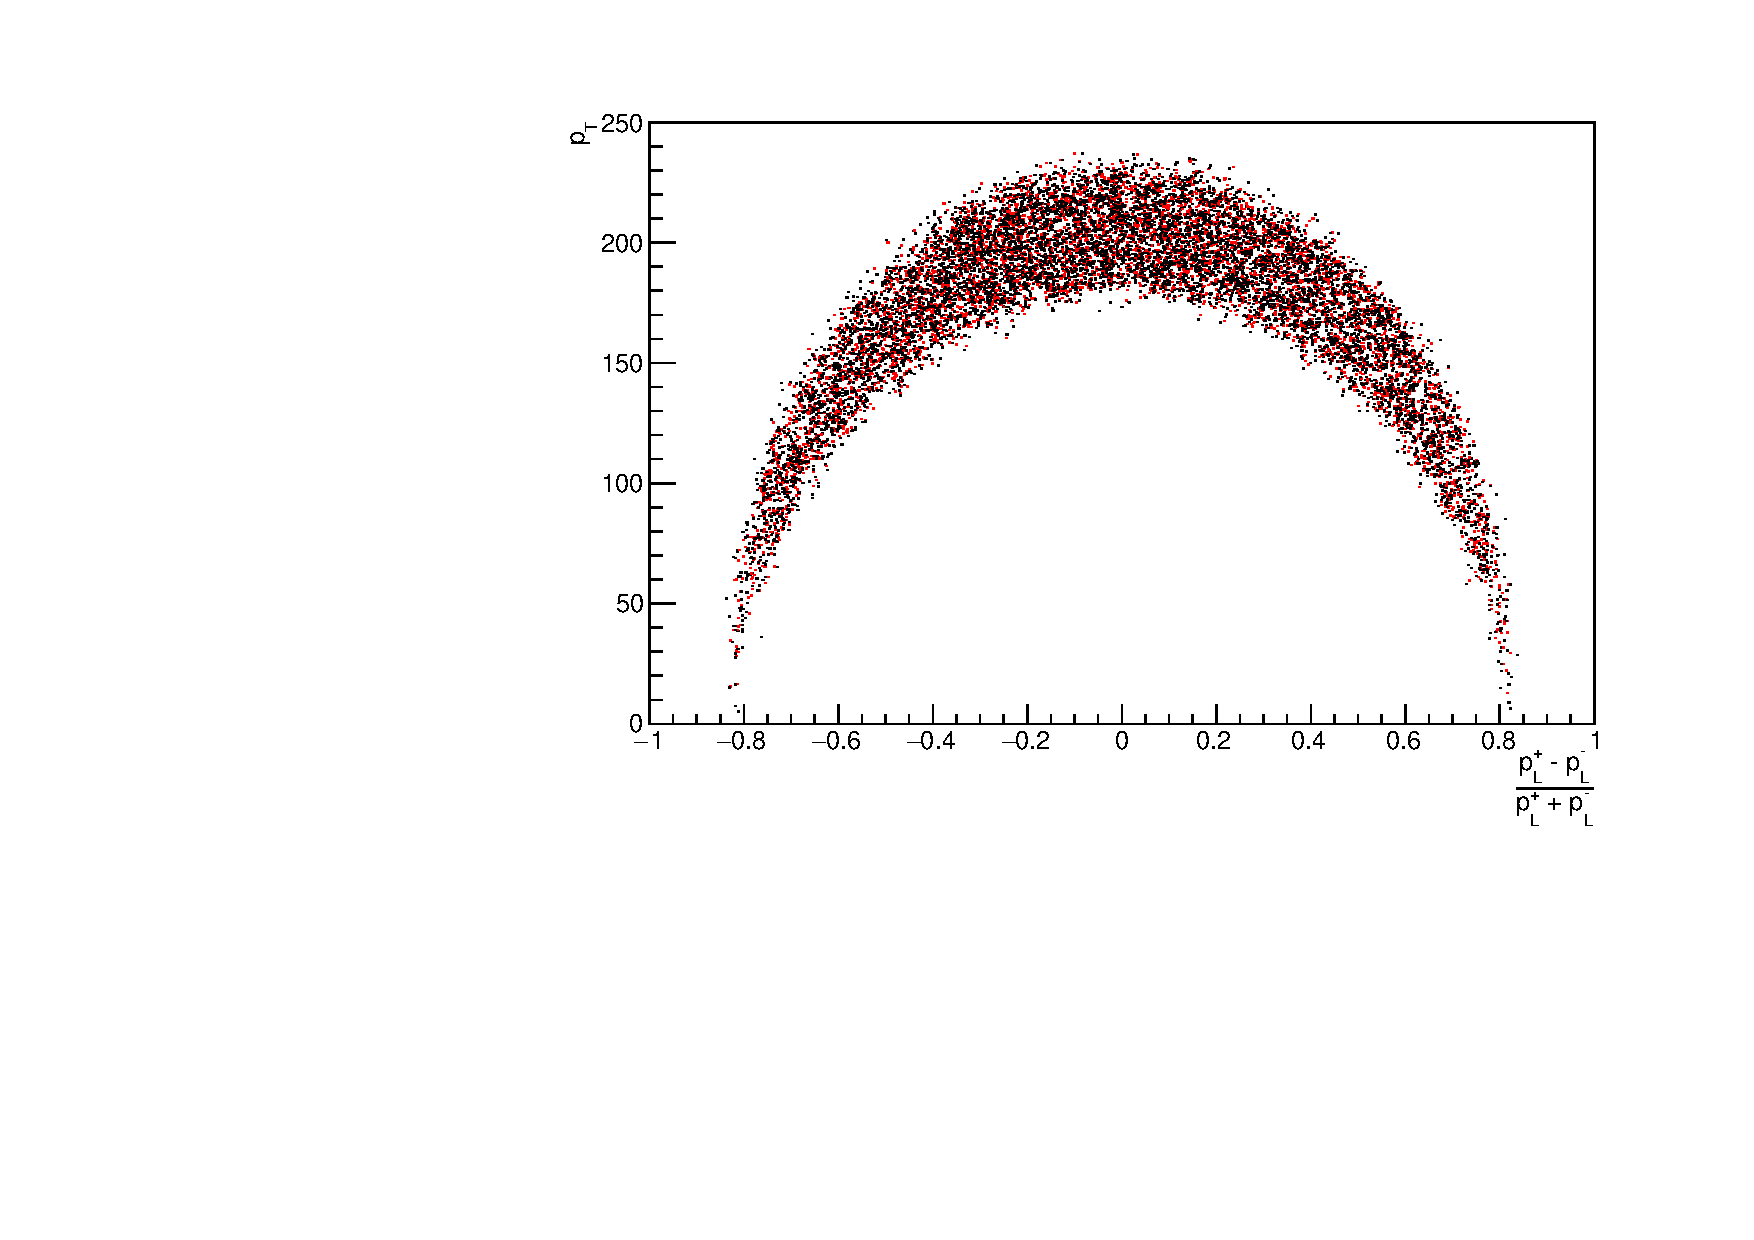
\includegraphics[width=0.5\linewidth]{figures/backgrounds/APplot_DD.pdf}
\put(-190,120) {(b)}
\caption{Armenteros-Podolanski plots for (a) LL, and (b) DD canididates. The $p_T$ values on the y axis are the transverse momentum of the daughters with respect to the mother particle and the x axis contains the longitudinal momentum asymmetry. The black points represent data and the red points represent MC.}
\label{applotsdata}
\end{figure}

\begin{figure}
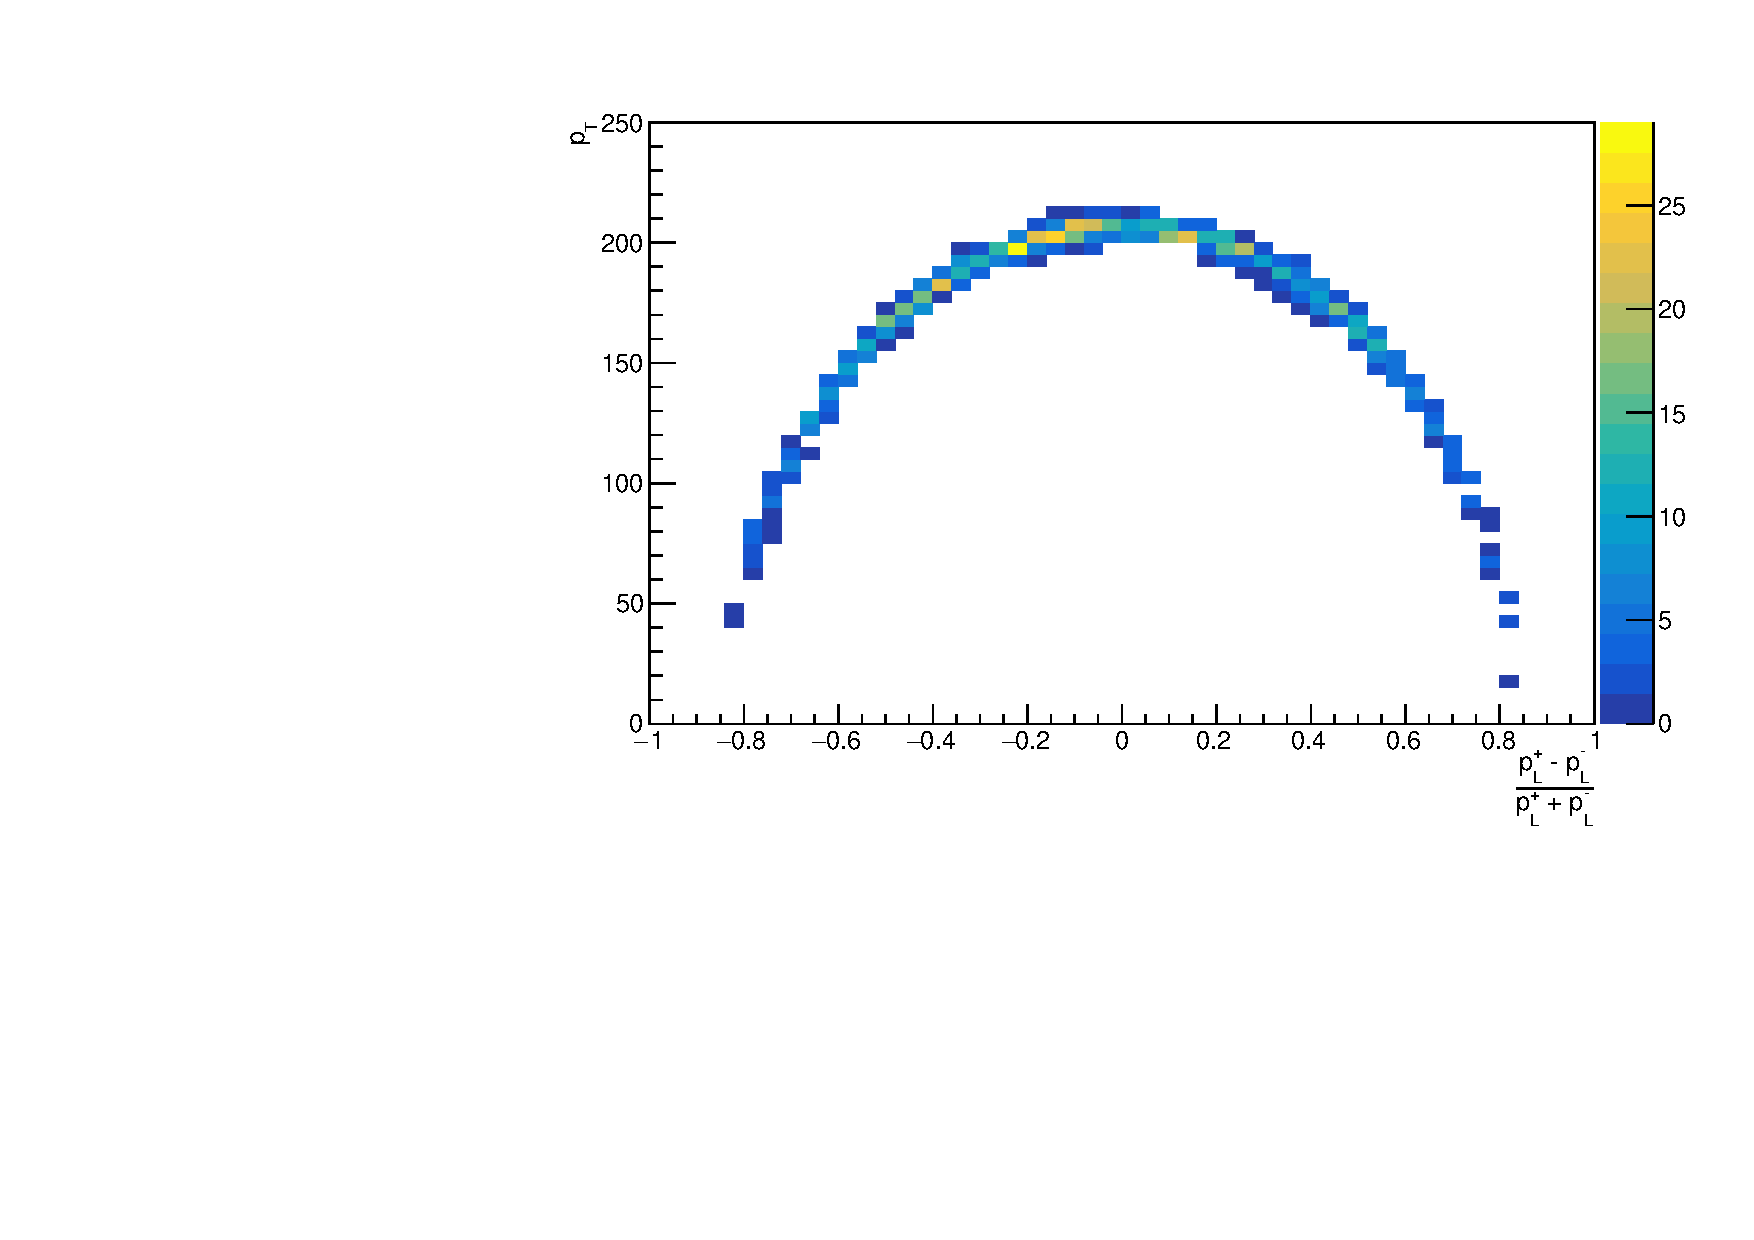
\includegraphics[width=0.5\linewidth]{figures/backgrounds/APplot_dataLL.pdf}
\put(-190,120) {(a)}
\hfill
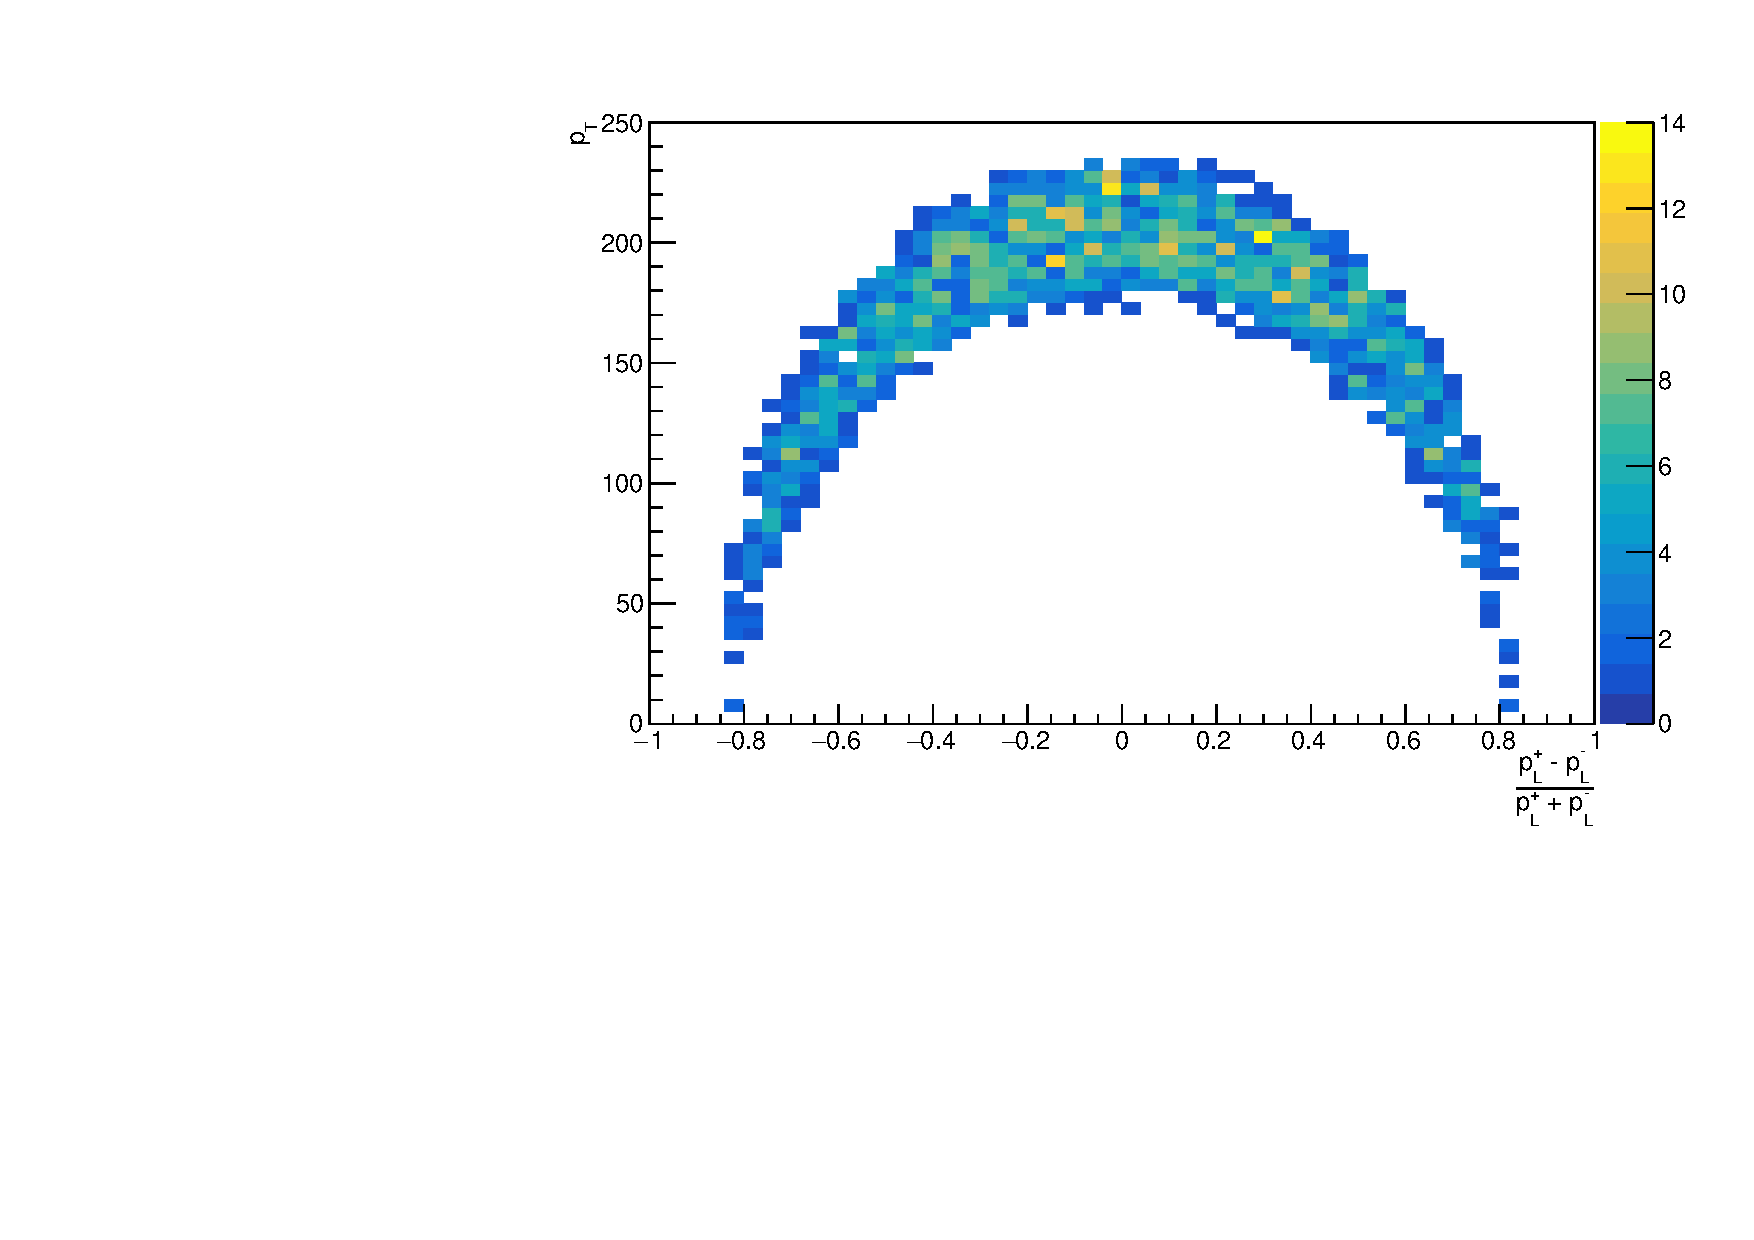
\includegraphics[width=0.5\linewidth]{figures/backgrounds/APplot_dataDD.pdf}
\put(-190,120) {(b)}
\caption{Armenteros-Podolanski plots for (a) LL, and (b) DD canididates in data. The $p_T$ values on the y axis are the transverse momentum of the daughters with respect to the mother particle and the x axis contains the longitudinal momentum asymmetry. The black points represent data and the red points represent MC.}
\label{applots}
\end{figure}

\begin{figure}
\centering
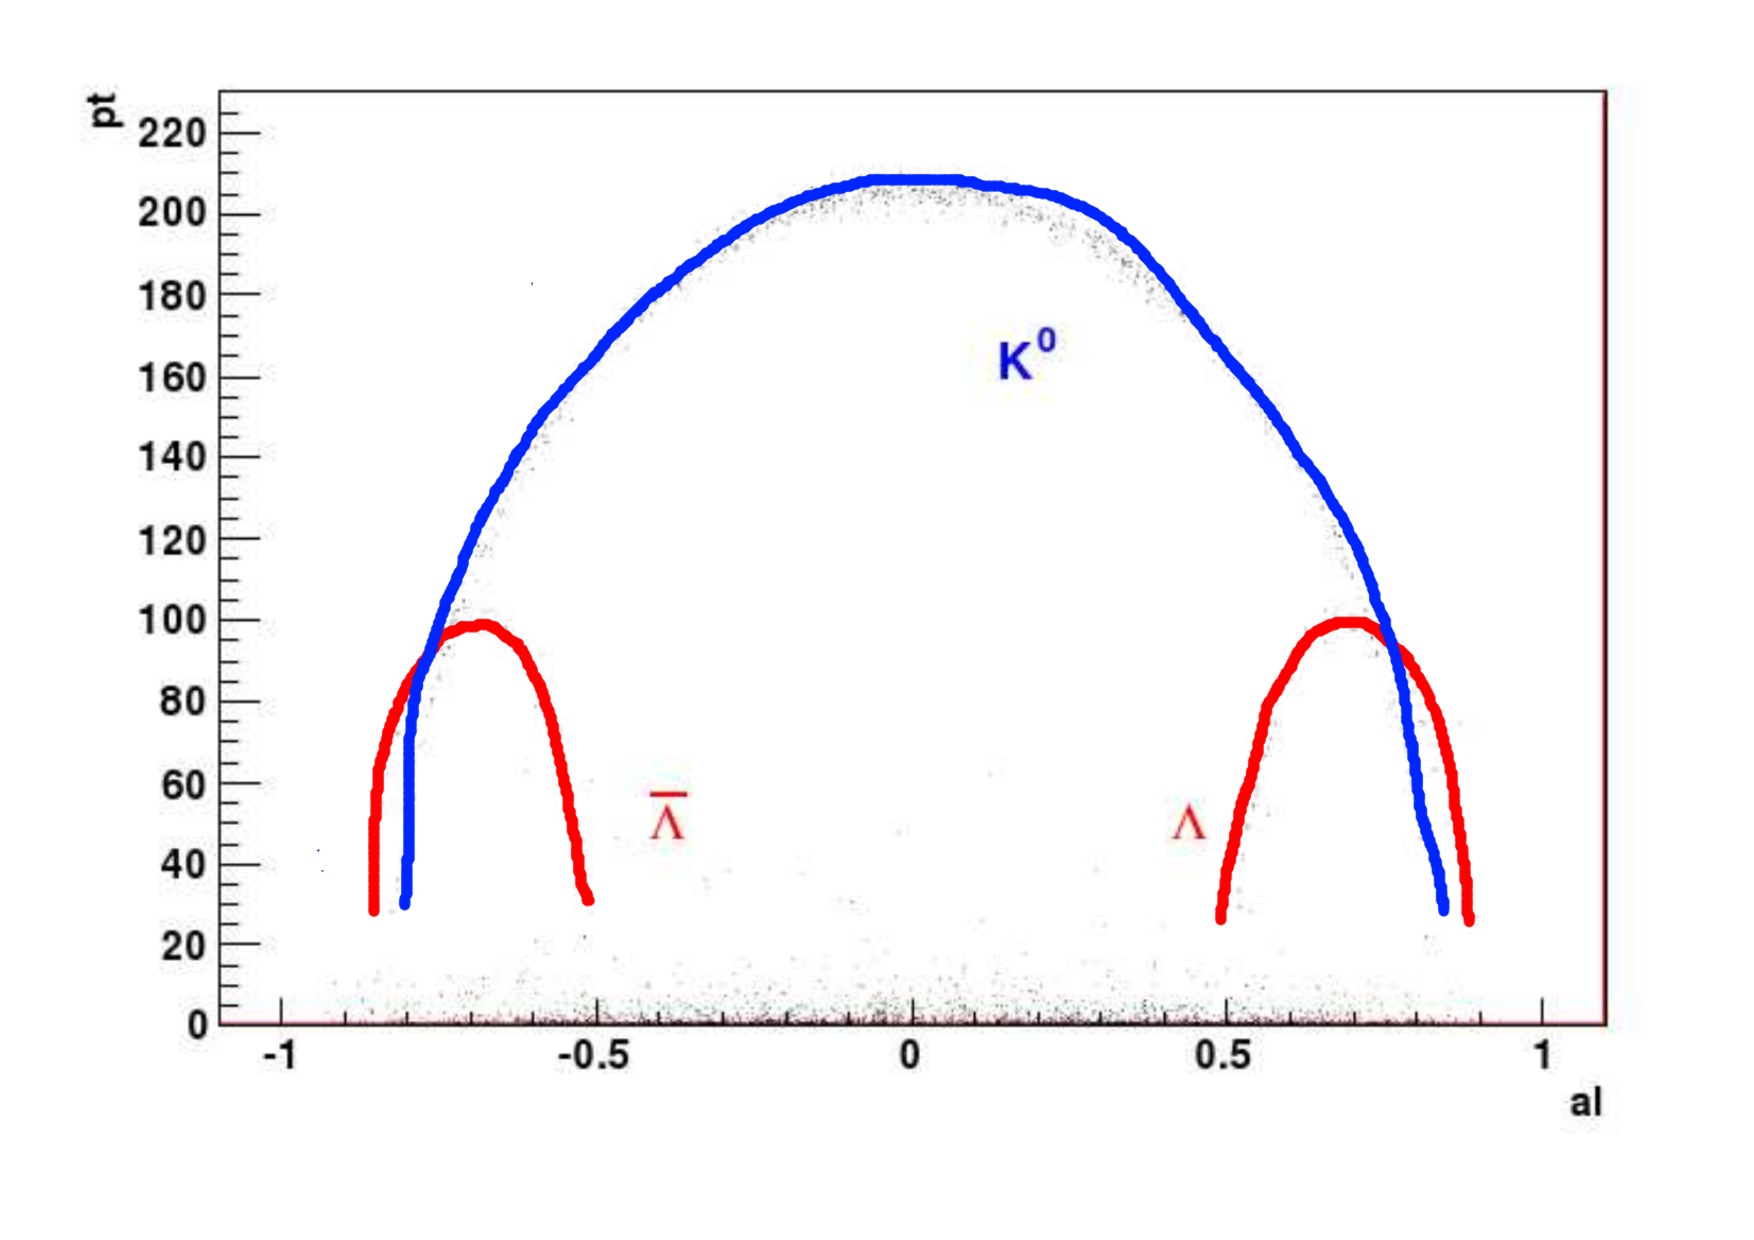
\includegraphics[width=0.5\linewidth]{figures/backgrounds/APfromPaper2.pdf}
\caption{An example Armenteros-Podolanski plot showing where the signal regions for \KS, \Lz and \Lbar are located in the AP plane~\cite{APplot}}
\label{apexample}
\end{figure}

\subsection{\decay{\B}{\D\KS\kaon}}
\label{sec:backgrounds:b2dkks}

The decay \decay{\B}{\D\KS\kaon} has a branching fraction of $5.5 \times 10^{-4}$~\cite{PDG2014}, which is similar to the signal branching fraction. However, nearly all of this background is removed by the 75 MeV \Kstarpm mass window and the DLLK $<$ 4 requirement on the bachelor pion. Table \ref{b2dkkspid} shows the rate of misidentification of the bachelor pion for \decay{\B}{\D\KS\kaon} MC.

\begin{table}[h]
\centering
\begin{tabular}{c|cc|cc}
\hline
& \multicolumn{2}{c}{LL} & \multicolumn{2}{c}{DD} \\
& MagUp & MagDown & MagUp & MagDown \\
\hline
2012 & $8.9 \pm 0.2$ & $8.1 \pm 0.2$ & $8.3 \pm 0.2$ & $8.0 \pm 0.2$ \\
2015 & $8.5 \pm 0.2$ & $9.7 \pm 0.2$ & $7.8 \pm 0.2$ & $7.4 \pm 0.2$ \\
\hline
Average Run 1 & \multicolumn{2}{c}{$8.5 \pm 0.3$} & \multicolumn{2}{c}{$8.2 \pm 0.3$} \\
Average Run 2 & \multicolumn{2}{c}{$9.1 \pm 0.2$} & \multicolumn{2}{c}{$7.6 \pm 0.3$} \\
\hline
\end{tabular}
\caption{MisID efficiencies for $B \to DK_sK$. The values in the table are given as percentages.}
\label{b2dkkspid}
\end{table}

Table \ref{b2dkkspid} shows that by requiring DLLK $<$ 4 on the bachelor pion the background is supressed to about 8\%. The efficiency of the 75 MeV \Kstarpm mass window when applied to \decay{\B}{\D\KS\kaon} MC is 3\% for both LL and DD. Combined misID rate and selection efficiencies means the decay is negligible even if the PID performance in Run 2 is not identical. Any residual amount is investigated alongside the systematics for the residual low mass background in this region.


\subsection{Other backgrounds}

Other backgrounds have been looked into and shown to have negligible contribution; a summary of these is given in Table \ref{ignoredbackgrounds}. No branching ratio has been measured for \decay{\Bm}{\Dz\Kstarm\piz} and \decay{\Bs}{\Dz\KS\pi\pi}, upper limits are guestimated hence this gives further motivation for restricting the mass range to 5230 \mevcc. As these backgrounds are estimated to have a low contribution in an area outside the mass range chosen for the \CP fit, they are considered negligible.

\begin{table}[h]
\centering
\begin{tabular}{cccc}
\hline
Decay mode & BR & Events relative to signal yield & Mass range (MeV) \\
\hline
\decay{\Bm}{\Dz\Kstarm\piz} & $6 \times 10^{-4}$ & 0.037/0.049 & 4750-5150 \\
\decay{\Bs}{\Dz\KS\pi\pi} & $5 \times 10^{-4}$ & 0.004/0.003 & 4750-5120 \\
\hline
\end{tabular}
\caption{Summary of background that have been investigated and determined to be negligible. Relative number of events are given for LL and DD (LL/DD). Branching ratios are guestimated upper limits}
\label{ignoredbackgrounds}
\end{table}

%In the \decay{\B}{Dh} analysis~\cite{LHCb-PAPER-2016-003}, the background \decay{\Lb}{\Lcm(\proton\Kp[\pim])\Kp} enters into the \decay{\Dz}{\Kp\Km} mode. This is where the \pim is missed in the reconstruction and the \proton is misIDed as a \kaon, this results in the recontructed \B mass falling within the mass fit range. This was found to be negligible and not affect the 

Many other backgrounds have been looked into and have been found to be negligible:

\begin{itemize}
\item \decay{\Bs}{\Dzb\Kstarz(\Kstarp[\pim])}
\item \decay{\Bs}{\Dstarp\Kstarp}
\item \decay{\Bs}{\Dspm(\kaon\kaon\pi)\Kstarpm}
\item \decay{\Bu}{\D\pi} with a random \KS added
\item \decay{\Bd}{\D\KS} with a  random pion added
\item \decay{\Bs}{\D\KS} with a random pion added
\item \decay{\Bu}{\D(\KS\pi\pi)\Kp}
\item \decay{\Lb}{\Lambda_c^-(\proton\Kp[\pim])\Kstarp} with the \proton misIDed as a kaon
\end{itemize}

\clearpage
